	\documentclass[10pt]{article}
\usepackage{graphicx}
\usepackage{float}
\usepackage[margin=.7in]{geometry}
\usepackage{amsmath}
\usepackage{caption}
\usepackage{subcaption}
\restylefloat{figure}
	\title{IT3708 - Exercise 2}
\author{
        Eirik Hammerstad \& Nicklas Utgaard
}
				
\date{\today}
\begin{document}
\maketitle
%\pagebreak
%\tableofcontents
%\pagebreak
\section{Description}
	\subsection{Architecture GA-core}\label{sec:core}
			Figure~\ref{fig:gastruct} below show the architecture of the core components for our evolutionary algorithm. The whole architecture is based around modularity and reusability, which can be seen by the abstract classes/interfaces named with italic font\footnote{\label{foot:abstractinterface}SelectionMechanism, SelectionProtocol, RangeBasedSelectionMechansim, StatisticsHandler, FitnessHandler, GenoType, PhenoType, Populationgenerator, PopulationParser}. This is a plain framework for solving problems through an evolitionary process and contains just the basics implementations for each interface, e.g. binary genotype, phenotype and populationgenerator, some selection mechanisms and protocols, and some population parsers in order to extract data from the process.
			
			The core architecture allows it to be used regardless of the problem specifics demands since these, as you will see in section~\ref{sec:specific}, are encoded into problem specific implementations of the abstract classes/interfaces\footnotemark[\ref{foot:abstractinterface}]
			\begin{figure}[H]
				\centerline{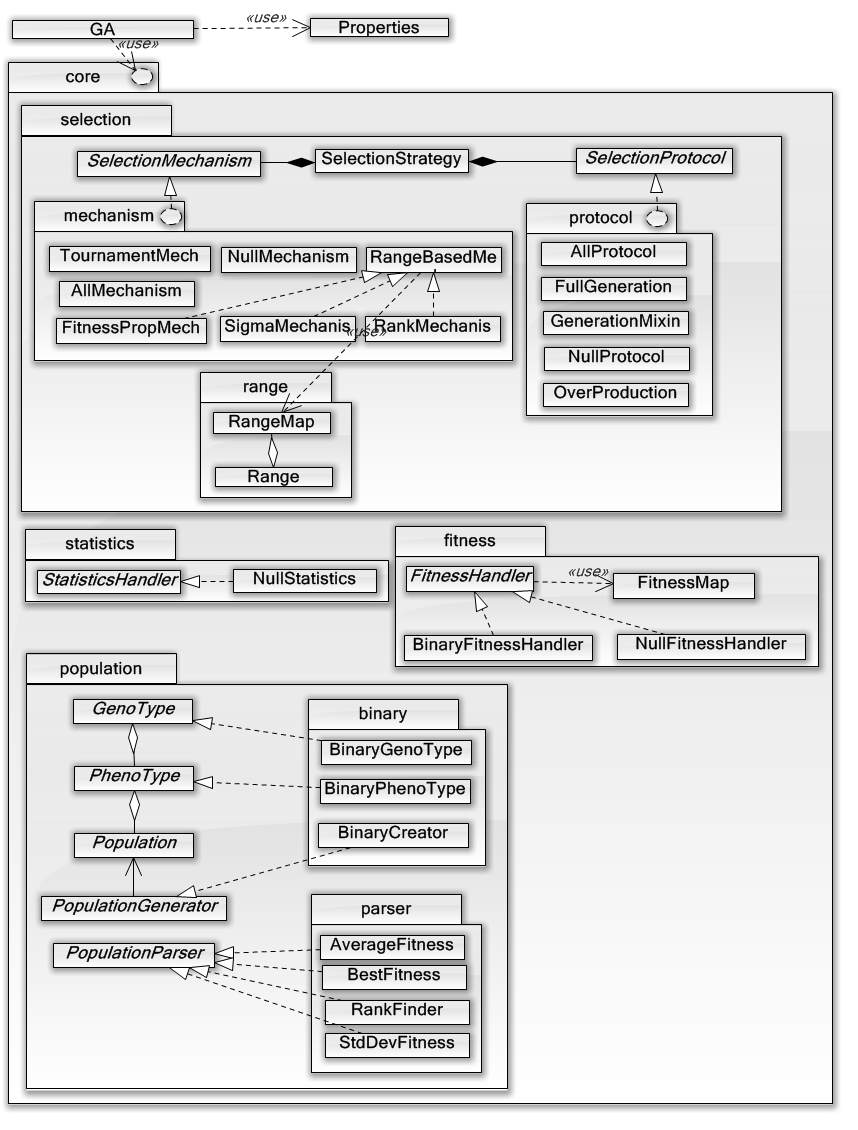
\includegraphics[width=.5\columnwidth]{./../images/GAStruct.png}}
				\caption{GA architecture}%
				\label{fig:gastruct}%
			\end{figure}

		\subsubsection{Problem specific}\label{sec:specific}
				In this exercise, we implement everything problem specific in a separate project. Our SpikeGenoType, SpikePhenoType, SpikeFitnessHandler and SpikePopulationCreator extends GenoType, PhenoType, FitnessHandler and PopulationGenerator from the core project respectivly.
		Our Spike project also implements an abstraction for the SpikeTrain, including functionality for different spike train distance metrics (waveform, spike time, spike interval), reading from file, and writing to file.
	\subsection{Genotype}\label{sec:geno}
		For the genotype representation we choose a discrete representation with cardinality $k~=~2$ and accuracy $acc$, which is decoded by the phenotype into the correct range based on which parameter the bit sequence is describing. The accuracy is an integer between 1 and 31, whihc determinds how many bits should be used to encode each parameter. The set of parameters for Izhikevich model each has it own range, described by $range_{param} \in [min_{param}, max_{param}]$. 
		\begin{align}
			range_a &\in [0.001, 0.2]\nonumber\\
			range_b &\in [0.01, 0.3]\nonumber\\
			range_c &\in [-80, -30]\nonumber\\
			range_d &\in [0.1, 10]\nonumber\\
			range_k &\in [0.01, 1.0]\nonumber
		\end{align}
		The conversion between the binary vector into real valued parameter is done by taking $acc$ bits and converting them to an integer $coef_{param}$. $subvector(bitvector, param)$ extracts the parameter relevant bits from the genotype bitvector.
		\begin{align}
			param &\in \{a, b, c, d, k\}\nonumber\\
			acc &= 8\nonumber\\
			bitvector &= 00001101\dots11100110\nonumber\\
			bitvector_{param} &= subvector(bitvector, param)\nonumber\\
			coef_{param} &= (bitvector_{param})_{10}\nonumber\\
			step_{param} &= (max_{param}-min_{param})/2^{acc}\nonumber\\
			param &= min_{param}+(coef_{param}*step_{param})\nonumber
		\end{align}
	\subsection{Fitness function}\label{sec:fitness}
		Our fitness function is based on the different SDM's implemented during this project, where $F_j$ is the phenotype in question, and $E_j$ the error found by the SDM associated with $F_j$.
		\begin{align}
			Fitness(F_j) &= \frac{1}{1+E_j}\nonumber
		\end{align}
\section{Test cases}\label{sec:test}
	The twelve test cases can be found below. The figure to the left show the target spike train in red and the best case spike train found with a given SDM in blue. The figure to the right show the fitness progression throughout the generations, with best fitness shown in green, average fitness in red, standard deviation of fitness in blue and the average entropy between the parameters for the entire population. All images is in addition added to the final delivery in order to make them visible in their original size. 
	
	In the parameters section for each of the datasets you can find the parameters used to configure the evolutionary algorithm, as well as the result parameter for our best case. The tree values for \textit{Avg Fitness} and \textit{SD} is the result of running our best case scenario twenty more times, with the time metric, interval metric and waveform metric respectively,  in order to see the average fitness generated by these parameters judged by the different SDM's.
	\subsection{Izzy 1}
		\subsubsection{Spike time distance metric}
			\begin{figure}[H]
				\centering
					\begin{subfigure}{.5\textwidth}
						\centering
						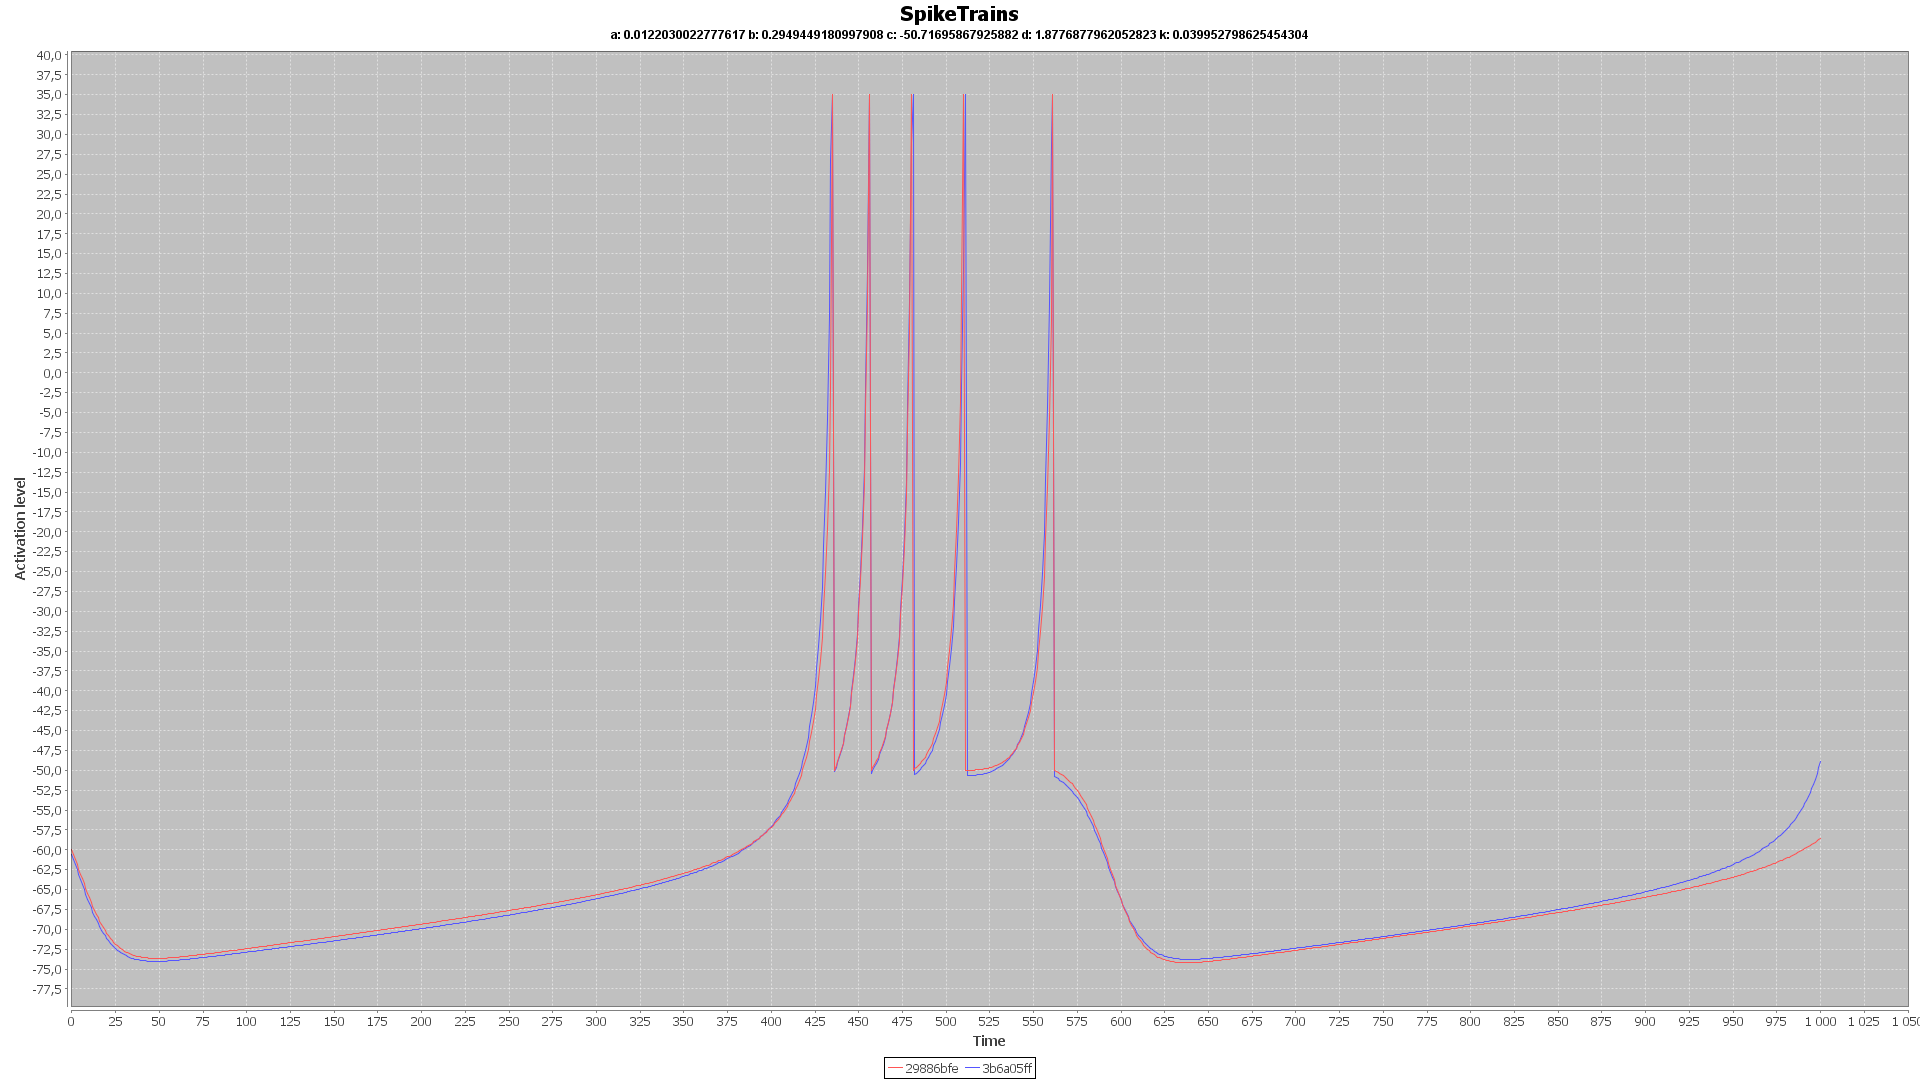
\includegraphics[width=\linewidth]{./../images/izzy1/time/plot.png}
						
						\label{fig:sub1a}
					\end{subfigure}%
					\begin{subfigure}{.5\textwidth}
						\centering
						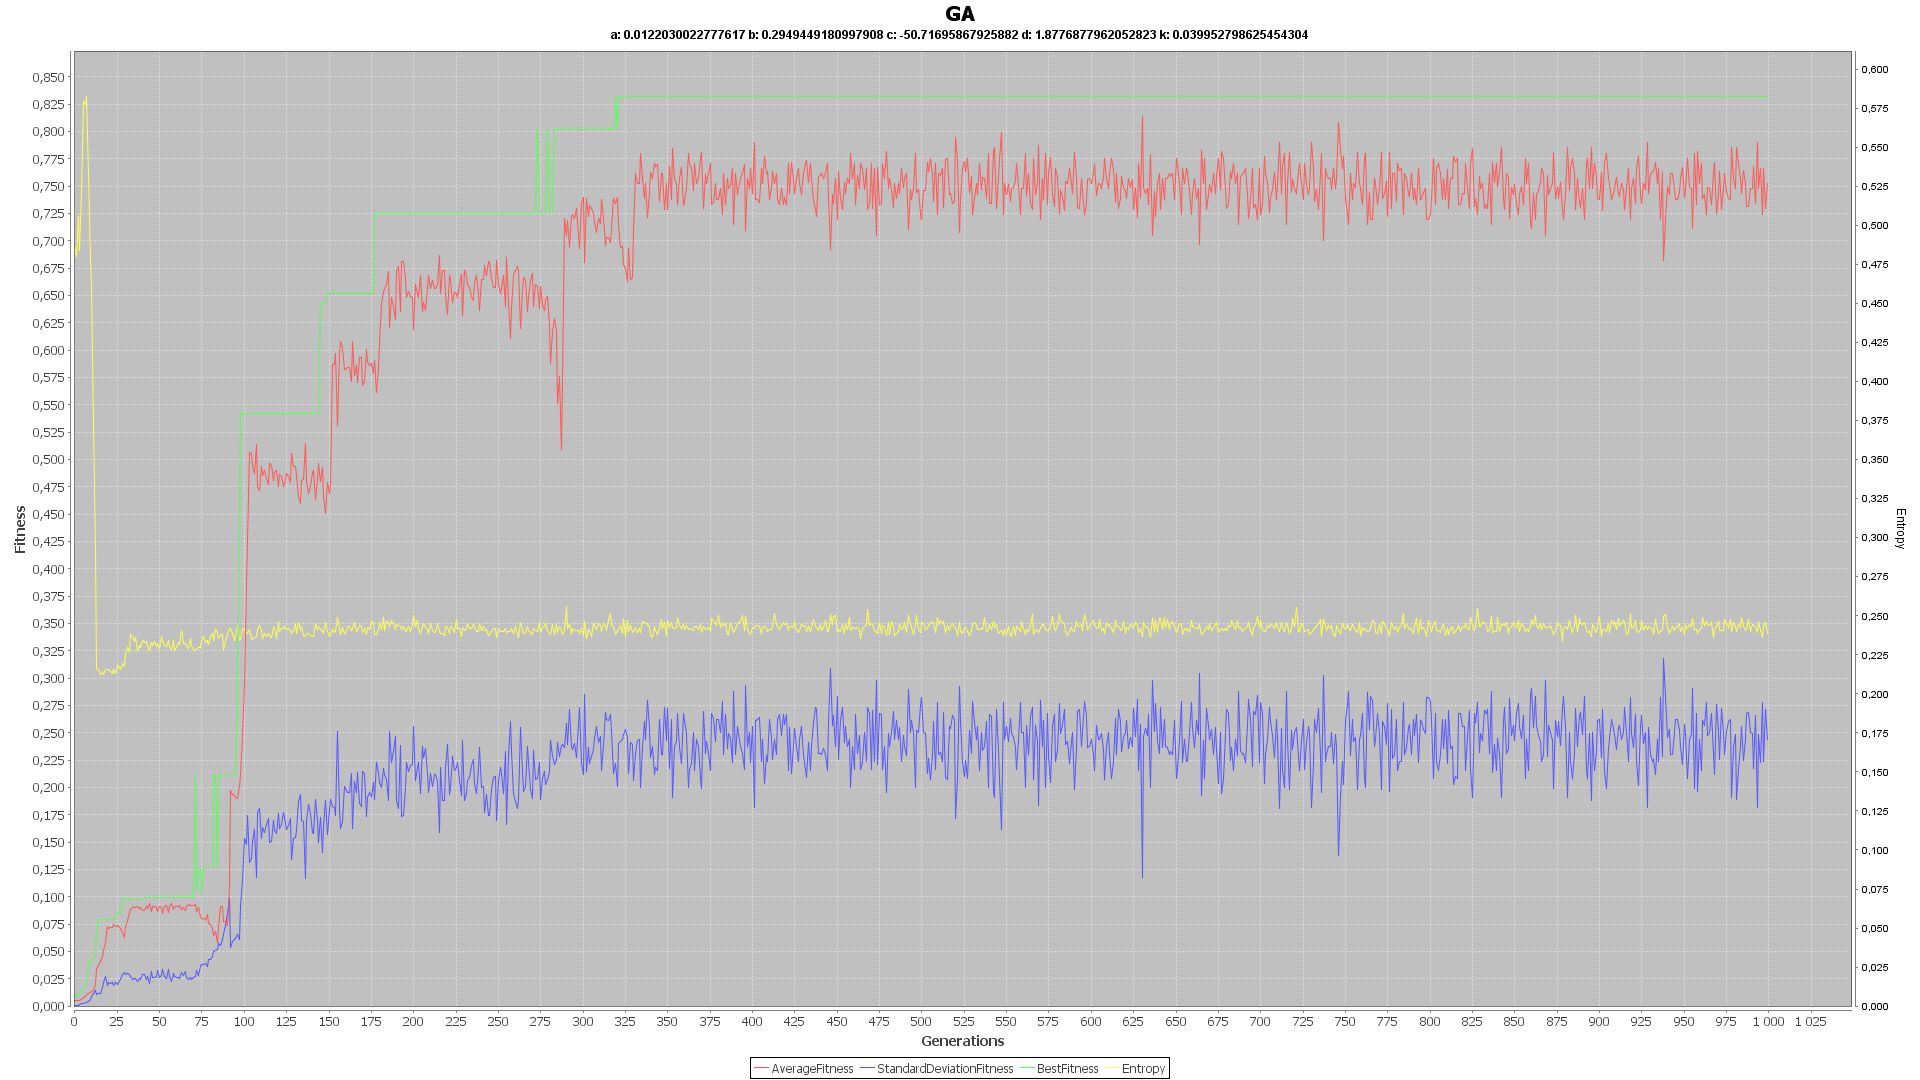
\includegraphics[width=\linewidth]{./../images/izzy1/time/prog.png}
						
						\label{fig:sub1b}
					\end{subfigure}
					
					\label{fig:plot1}
			\end{figure}
			
		\subsubsection{Spike interval distance metric}
			\begin{figure}[H]
				\centering
					\begin{subfigure}{.5\textwidth}
						\centering
						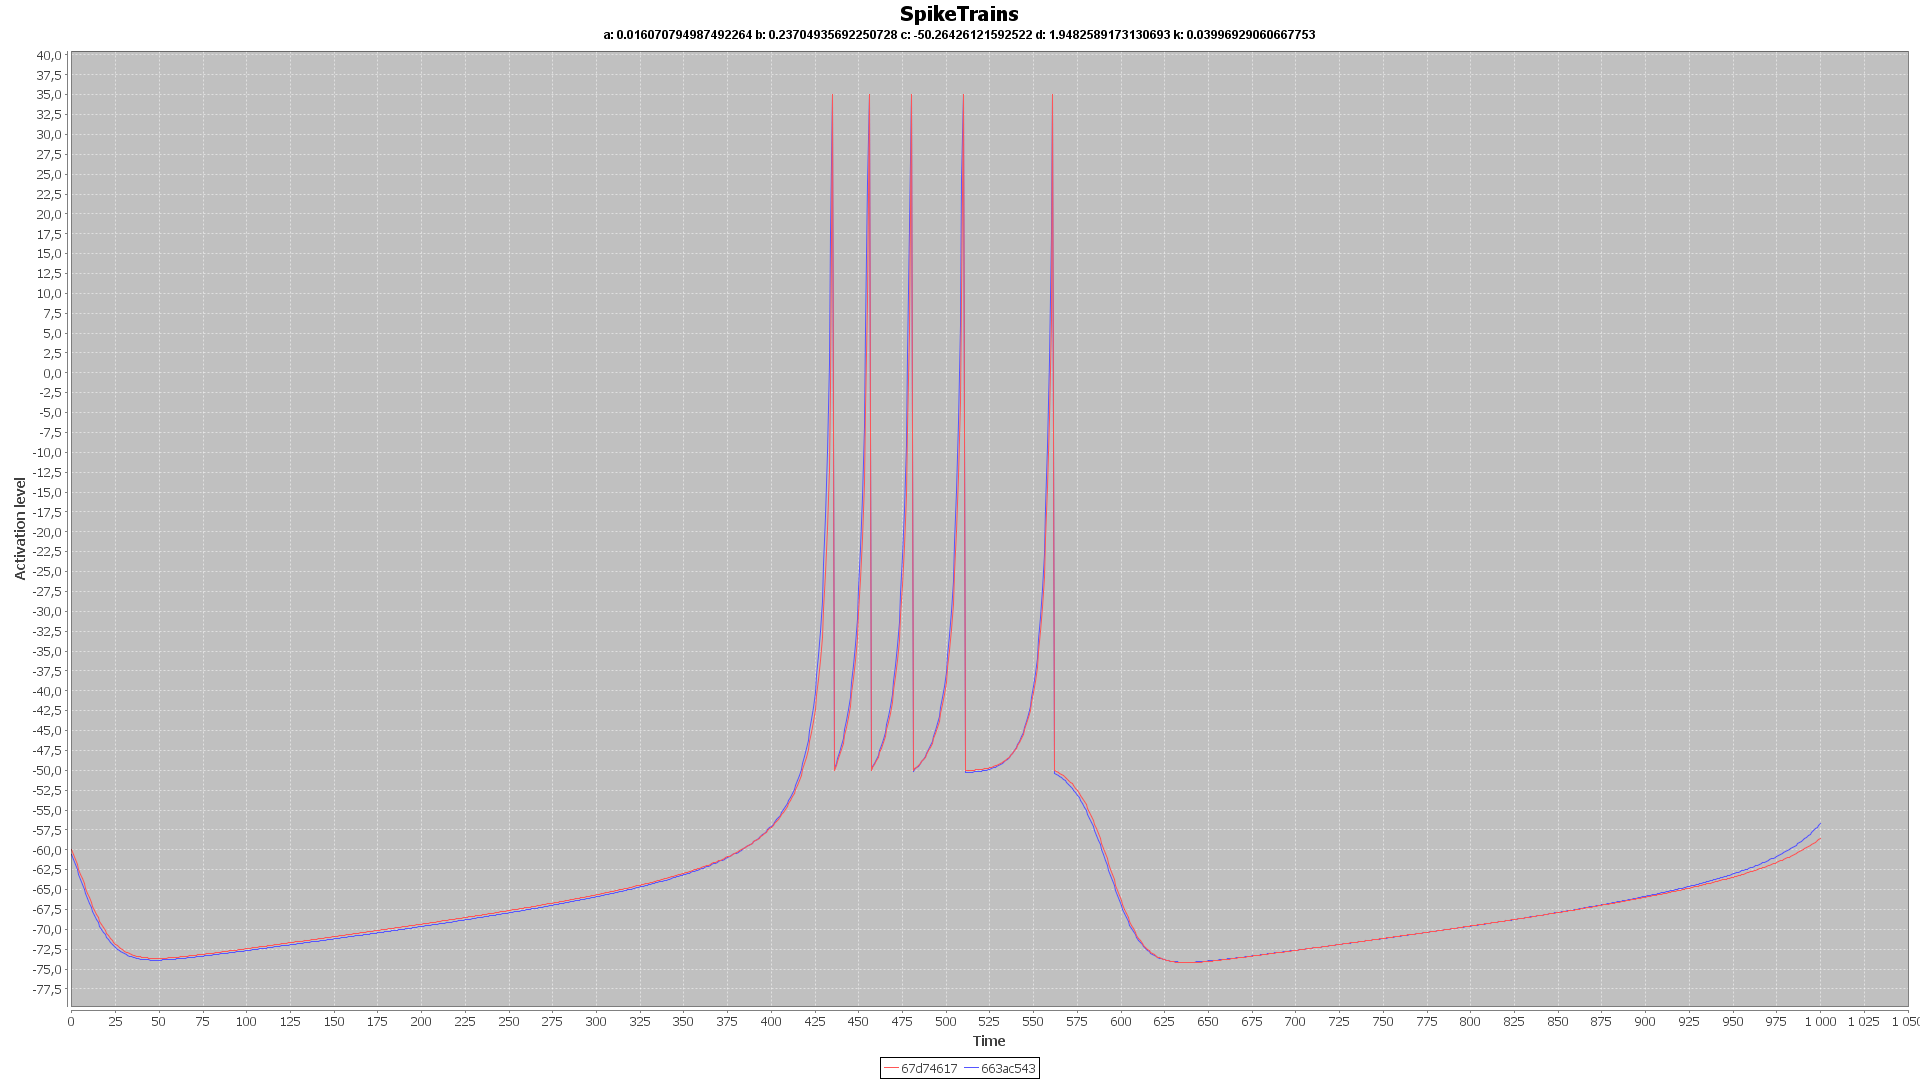
\includegraphics[width=\linewidth]{./../images/izzy1/interval/plot.png}
						
						\label{fig:sub2a}
					\end{subfigure}%
					\begin{subfigure}{.5\textwidth}
						\centering
						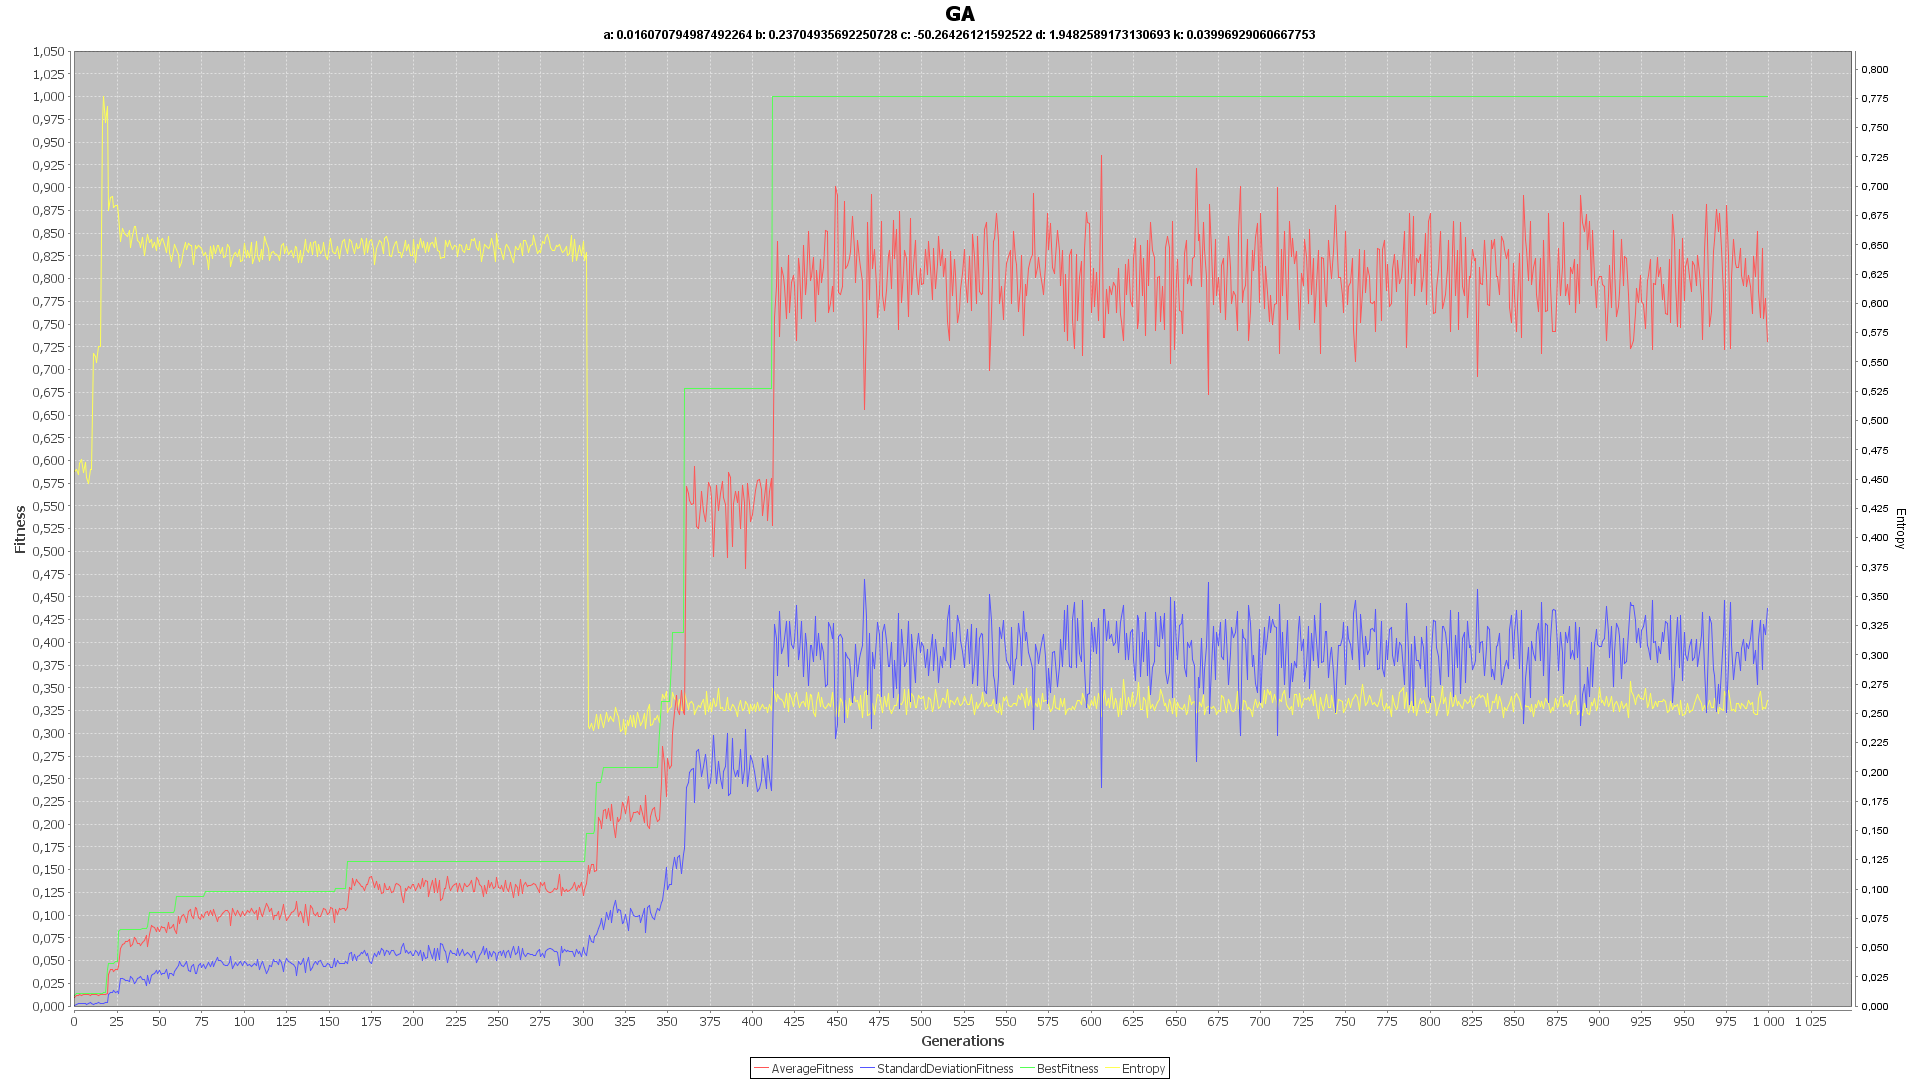
\includegraphics[width=\linewidth]{./../images/izzy1/interval/prog.png}
						
						\label{fig:sub2b}
					\end{subfigure}
					
					\label{fig:plot2}
			\end{figure}
		
		\subsubsection{Waveform distance metric}
			\begin{figure}[H]
				\centering
					\begin{subfigure}{.5\textwidth}
						\centering
						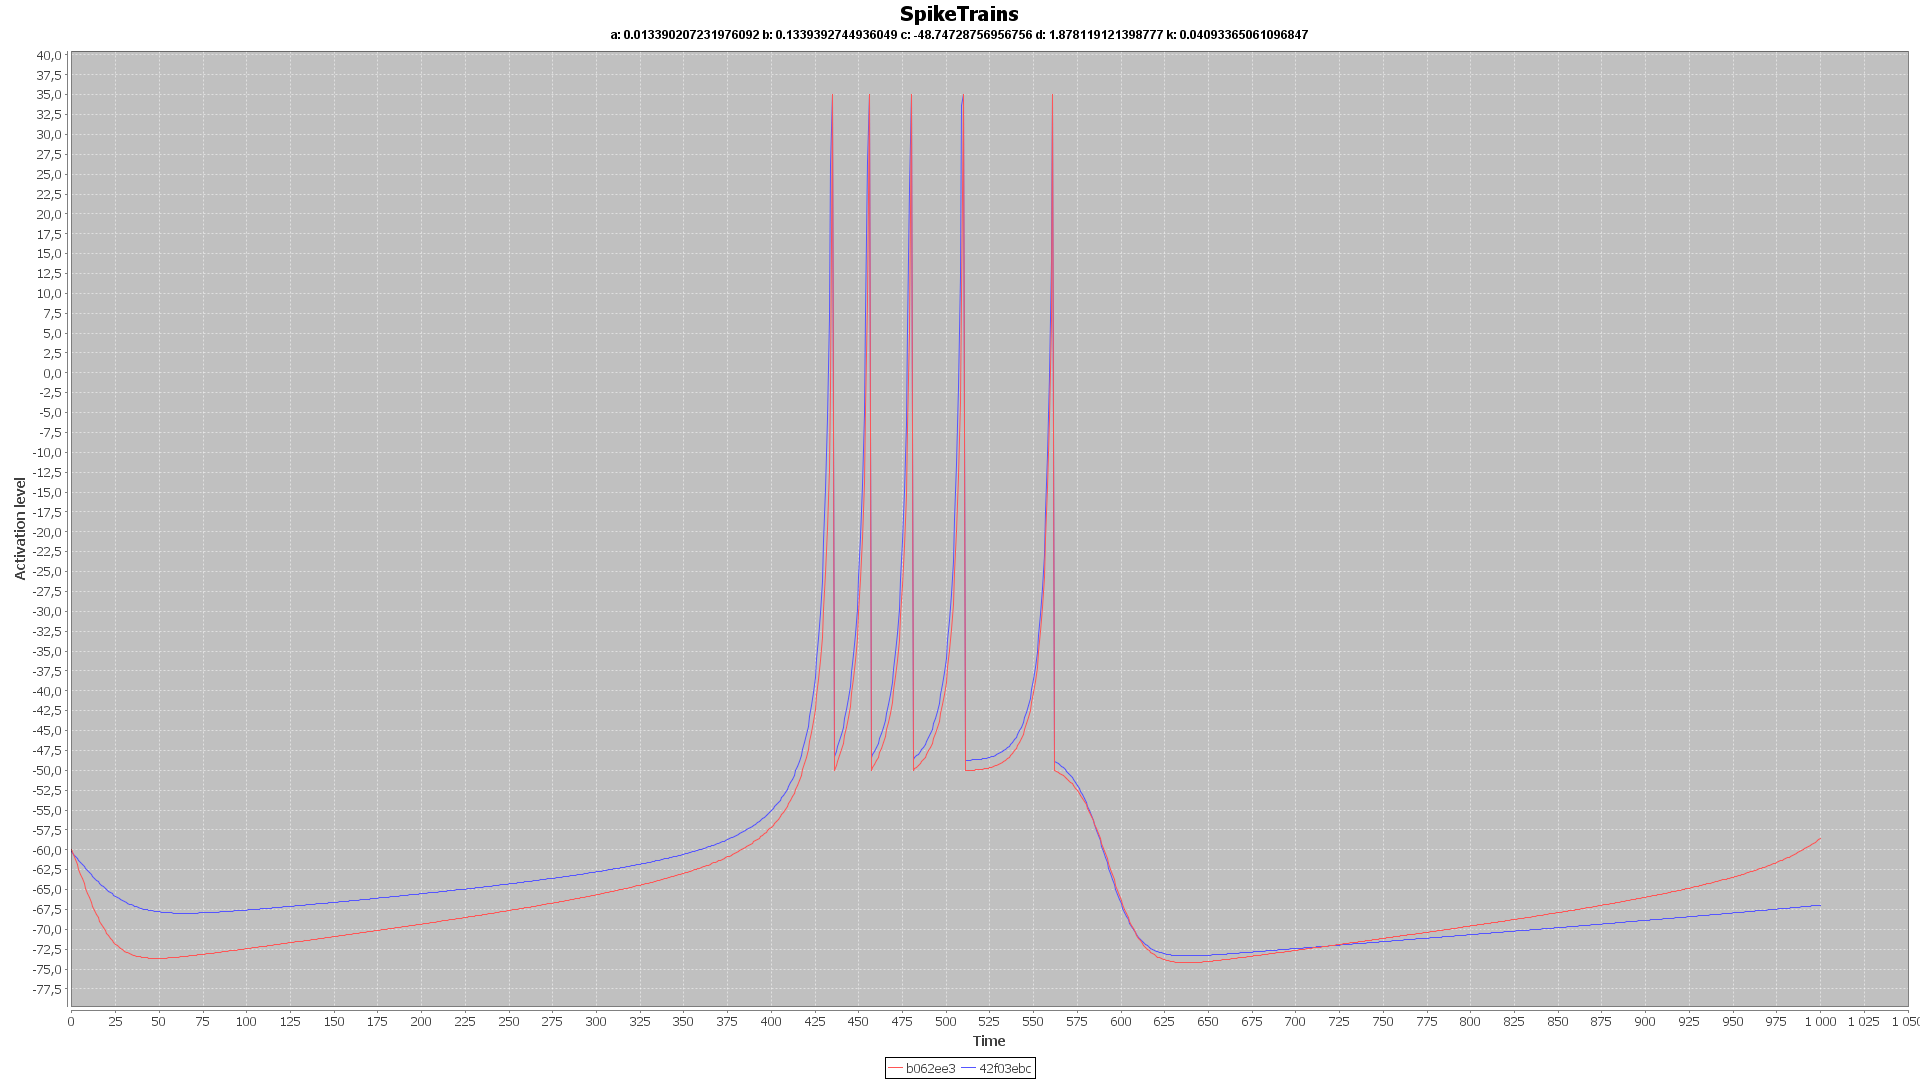
\includegraphics[width=\linewidth]{./../images/izzy1/wave/plot.png}

						\label{fig:sub3a}
					\end{subfigure}%
					\begin{subfigure}{.5\textwidth}
						\centering
						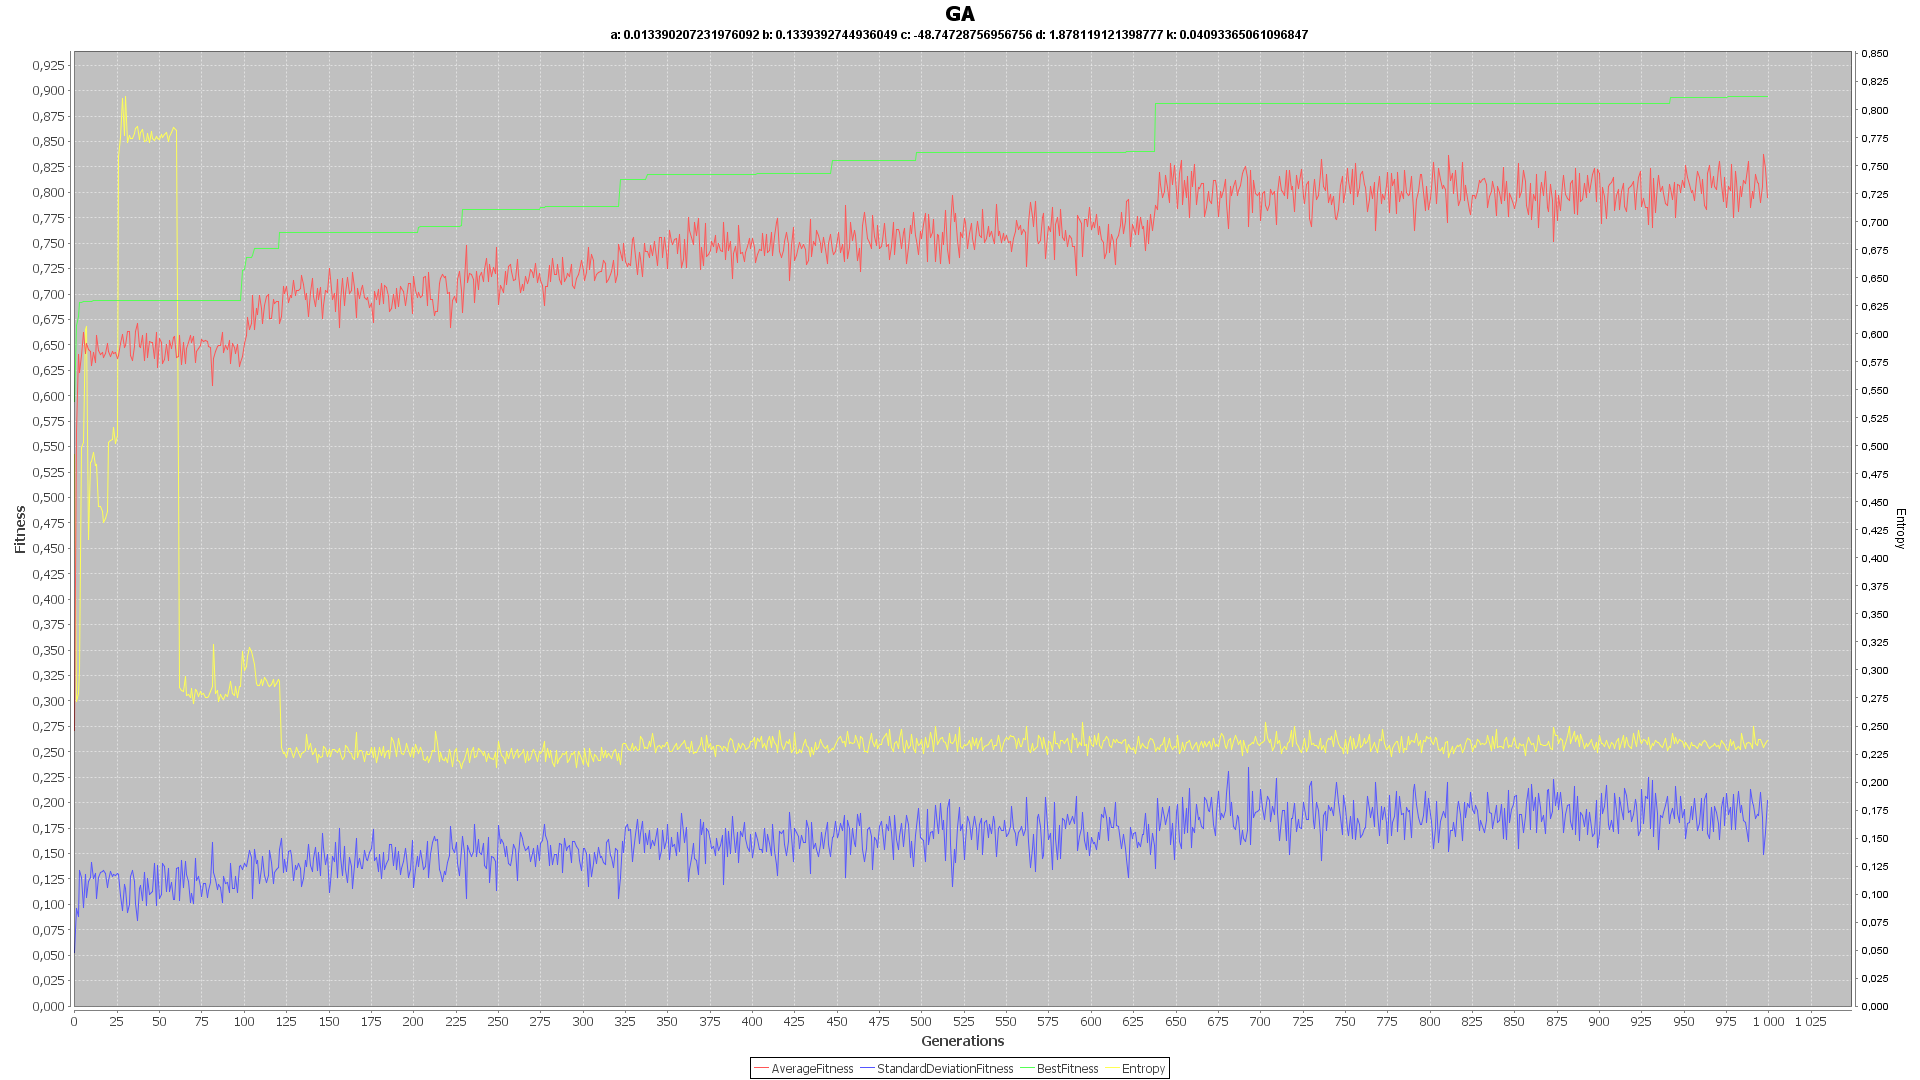
\includegraphics[width=\linewidth]{./../images/izzy1/wave/prog.png}
						
						\label{fig:sub3b}
					\end{subfigure}
					
					\label{fig:plot3}
			\end{figure}
		\subsubsection{Parameters}
			\begin{table}[H]
				\begin{tabular}{lll}
					SDM & Best Fitness & Parameter\\\hline\hline
					SpikeTime & $0.8319$ & $[a,b,c,d,k]= [0.0122,0.2949, -50.71, 1.878, 0.0399]$\\
					SpikeInterval & $1.0$ & $[a,b,c,d,k]= [0.0161,0.2370, -50.26, 1.948, 0.0399]$\\
					Waveform & $0.8939$ & $[a,b,c,d,k]= [0.0134,0.1339, -48.75, 1.878, 0.0409]$\\
				\end{tabular}
				\caption{The best found solutions for izzy 1 given the SDM}
			\end{table}
		
	\subsection{Izzy 2}
		\subsubsection{Spike time distance metric}
			\begin{figure}[H]
				\centering
					\begin{subfigure}{.5\textwidth}
						\centering
						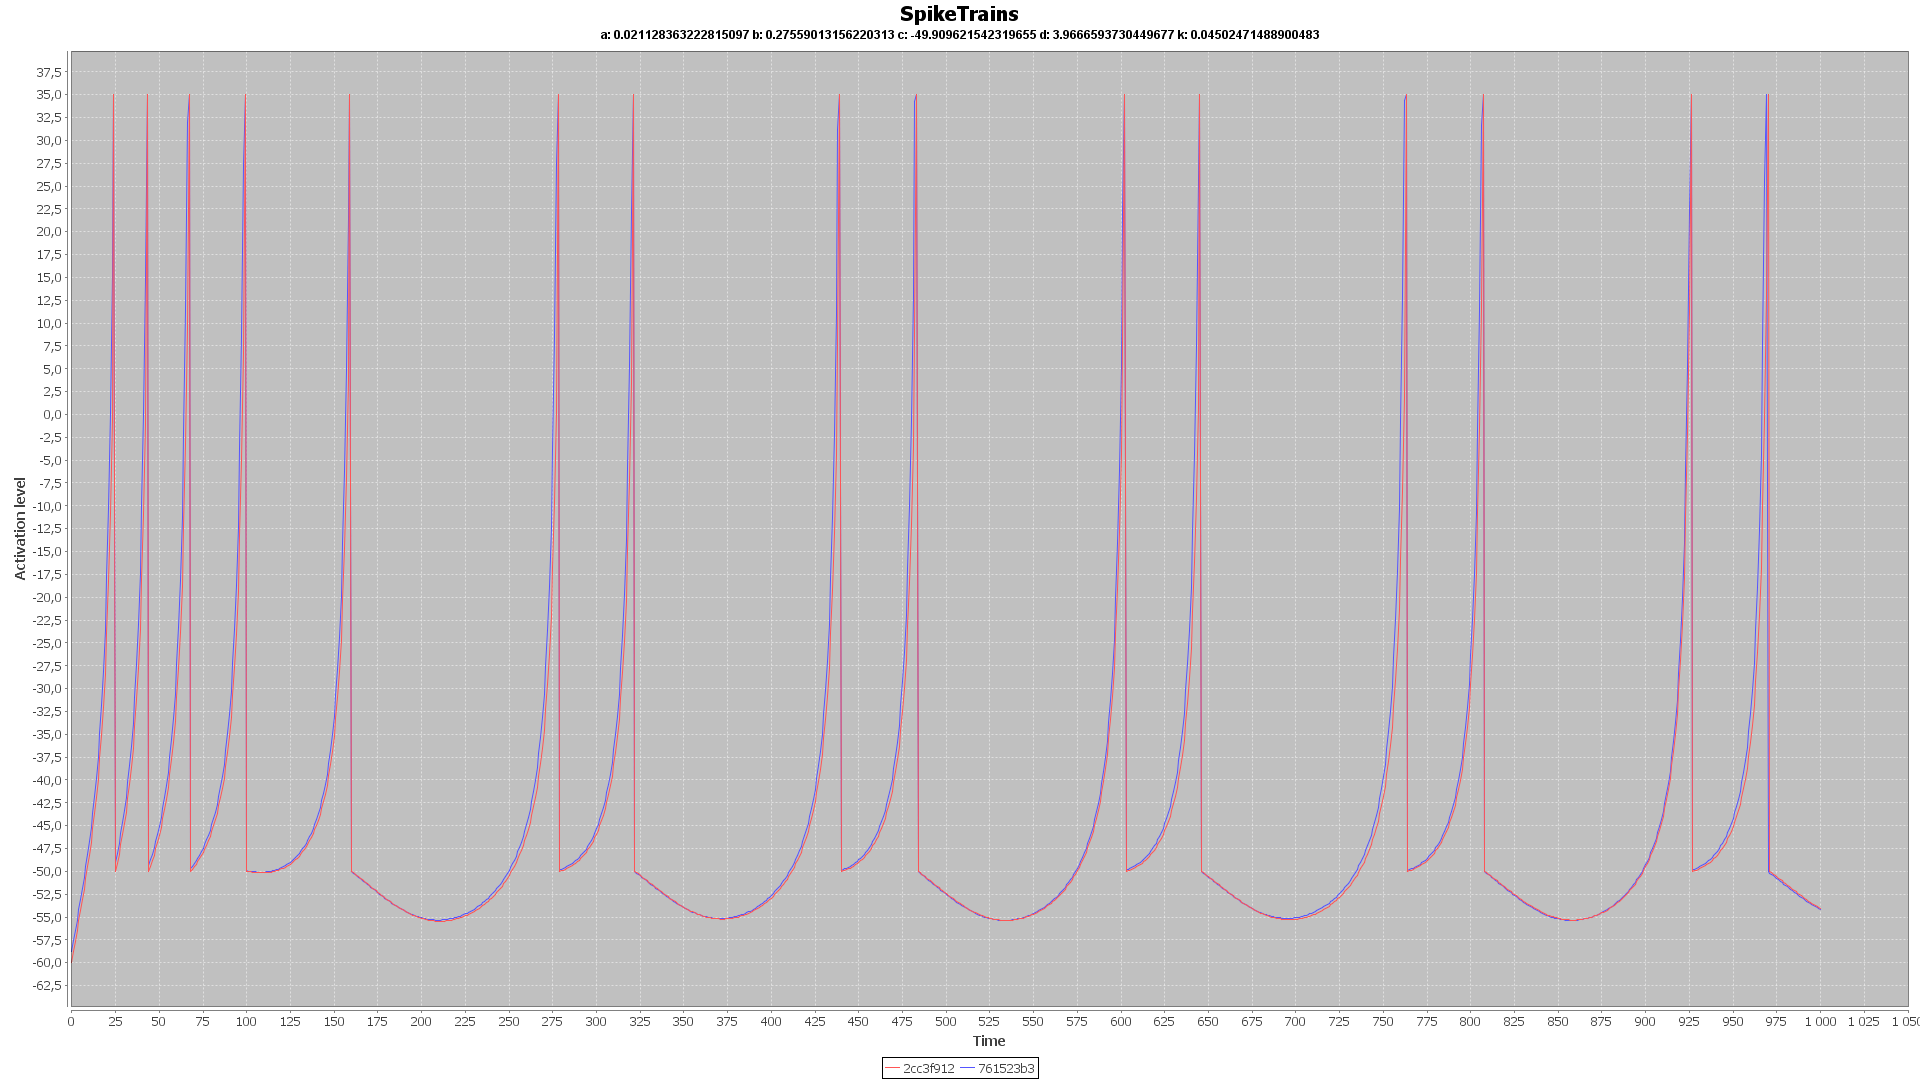
\includegraphics[width=\linewidth]{./../images/izzy2/time/plot.png}
						
						\label{fig:sub4a}
					\end{subfigure}%
					\begin{subfigure}{.5\textwidth}
						\centering
						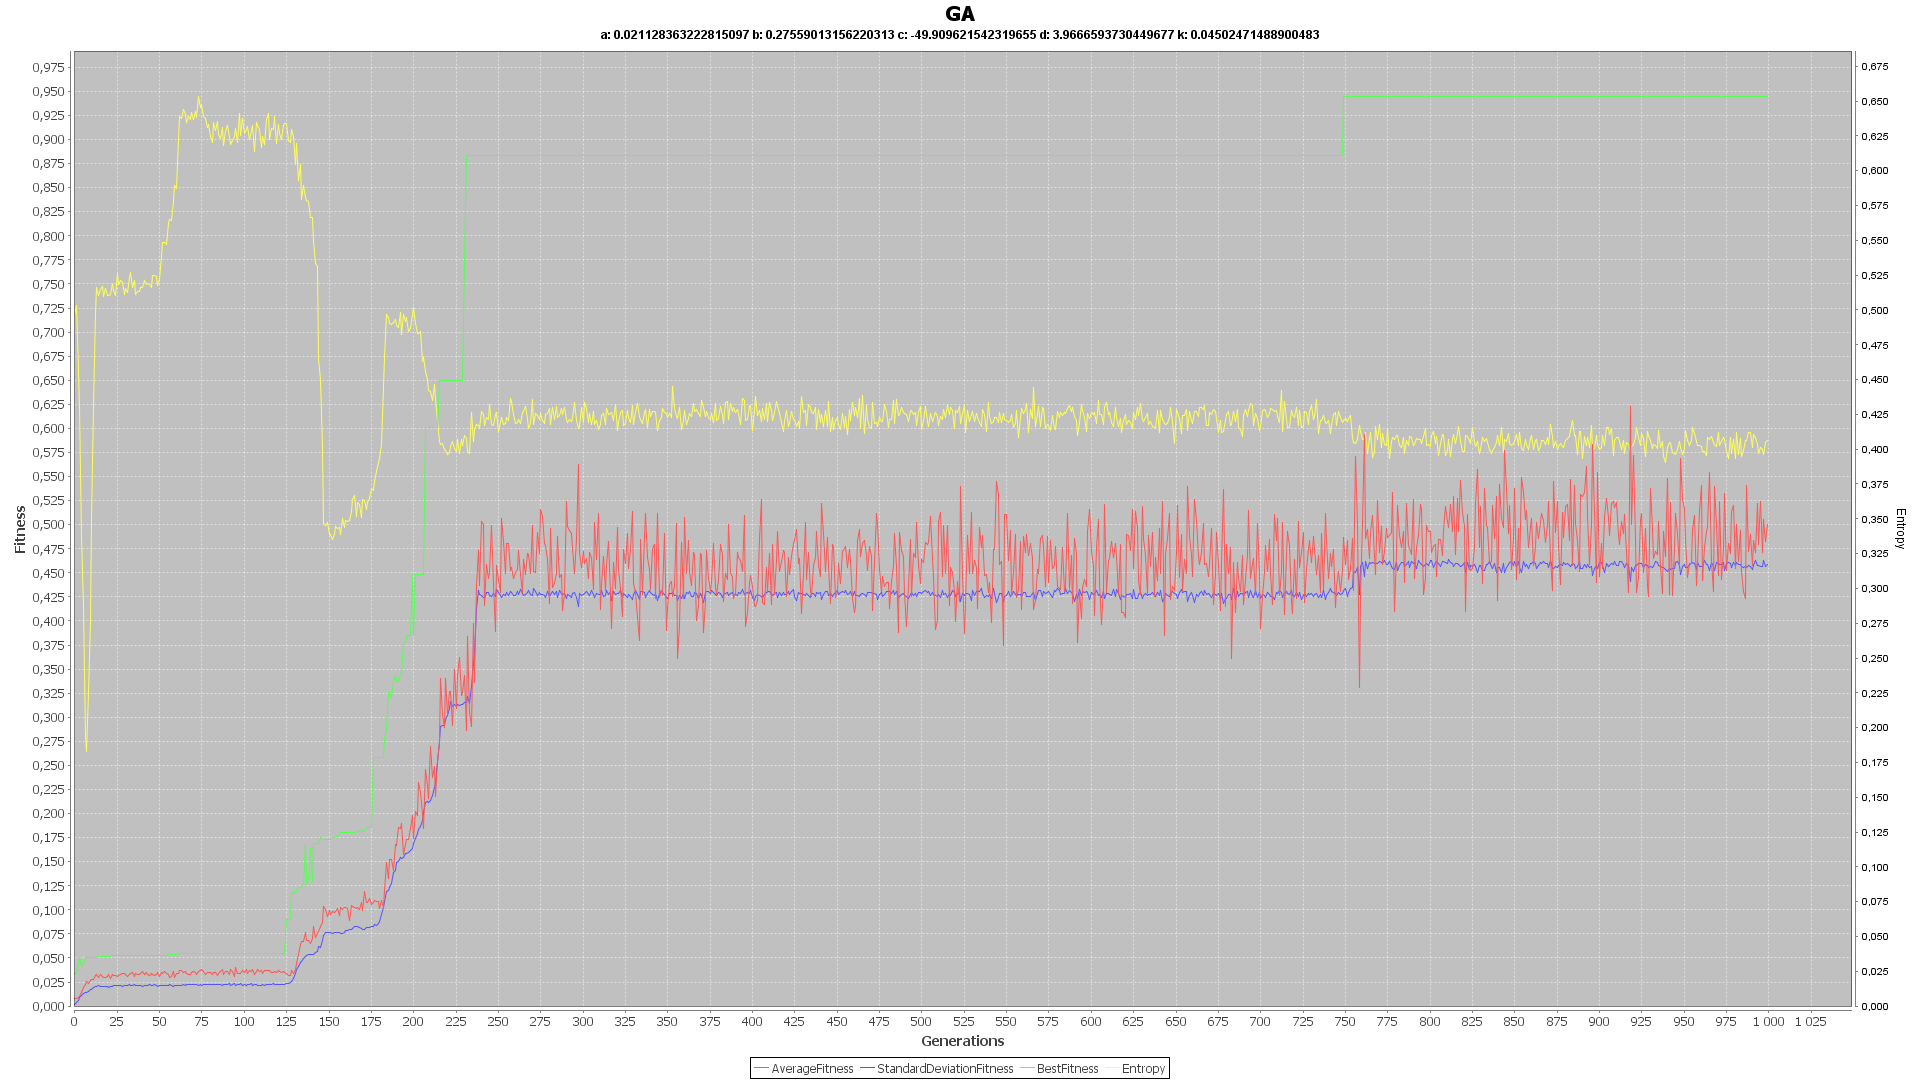
\includegraphics[width=\linewidth]{./../images/izzy2/time/prog.png}
						
						\label{fig:sub4b}
					\end{subfigure}
					
					\label{fig:plot4}
			\end{figure}
			
		\subsubsection{Spike interval distance metric}
			\begin{figure}[H]
				\centering
					\begin{subfigure}{.5\textwidth}
						\centering
						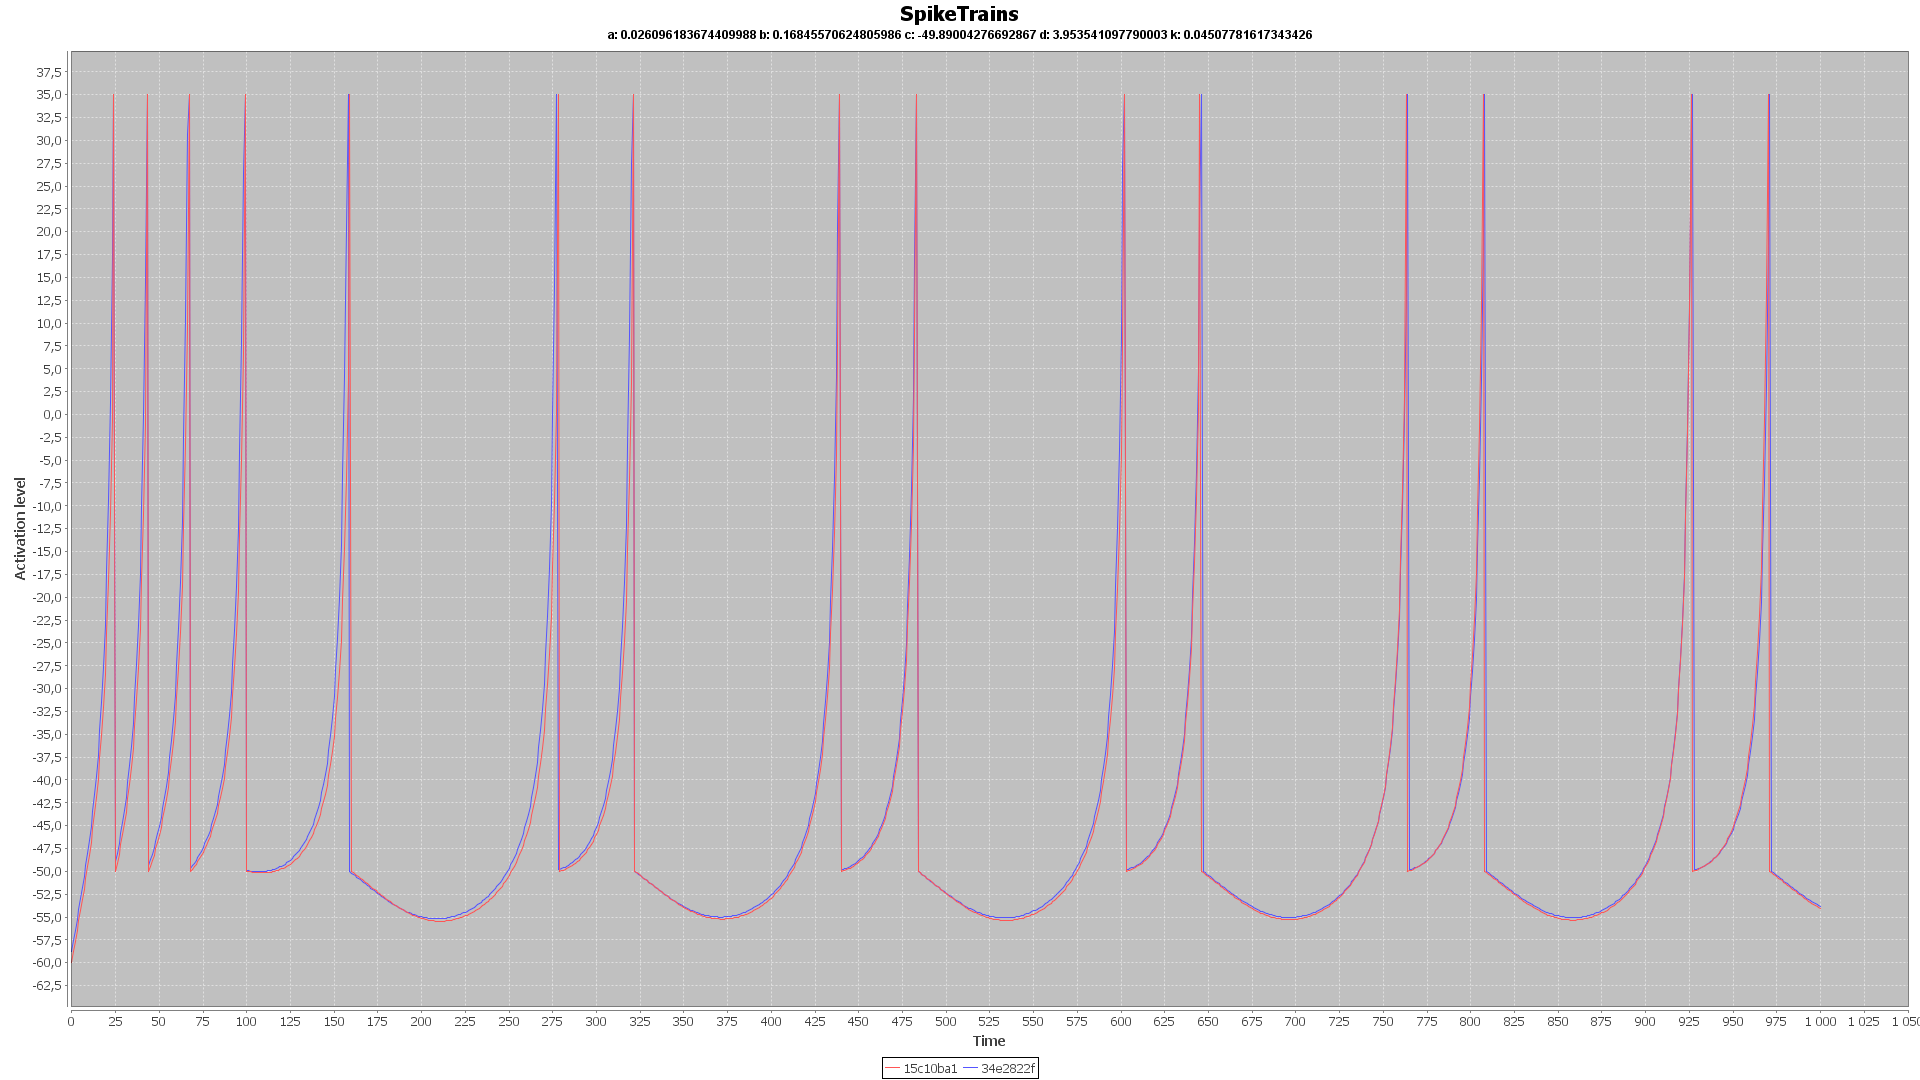
\includegraphics[width=\linewidth]{./../images/izzy2/interval/plot.png}
						
						\label{fig:sub5a}
					\end{subfigure}%
					\begin{subfigure}{.5\textwidth}
						\centering
						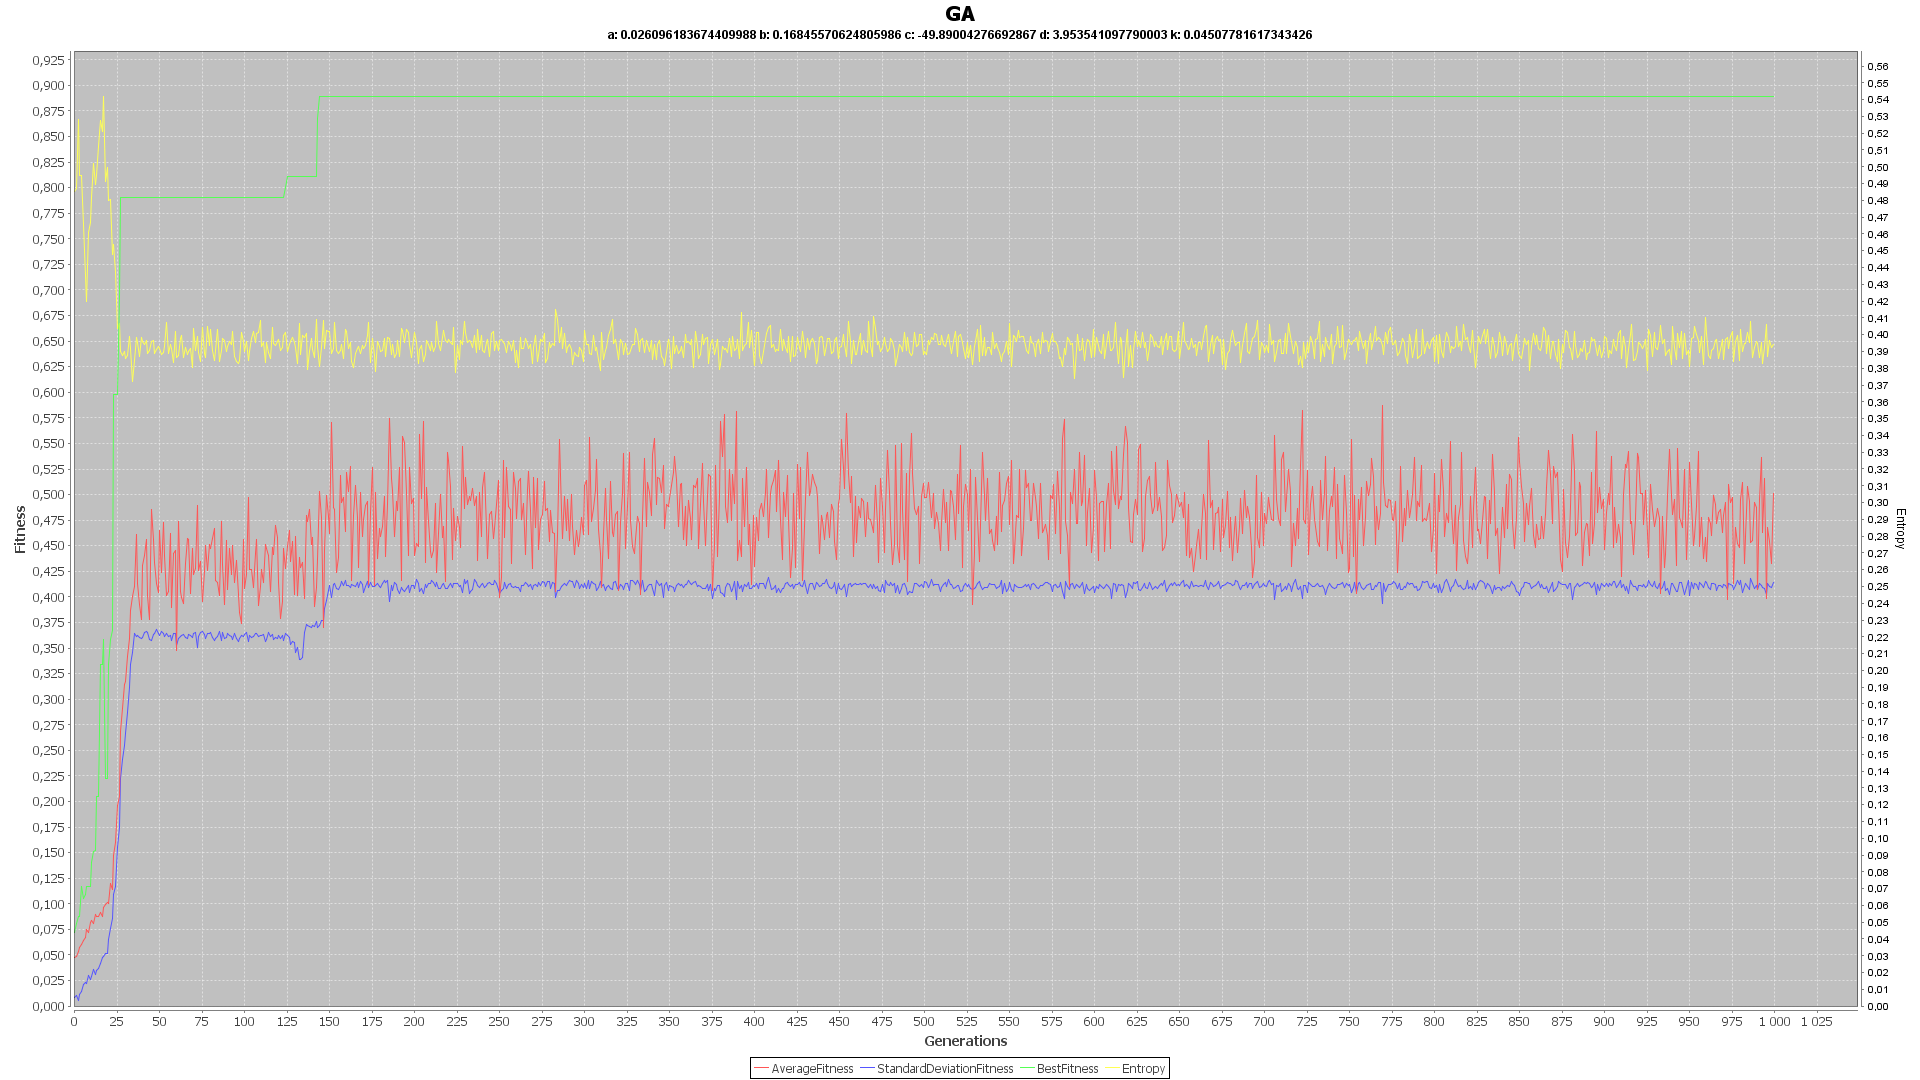
\includegraphics[width=\linewidth]{./../images/izzy2/interval/prog.png}
						
						\label{fig:sub5b}
					\end{subfigure}
					
					\label{fig:plot5}
			\end{figure}
			
		\subsubsection{Waveform distance metric}
			\begin{figure}[H]
				\centering
					\begin{subfigure}{.5\textwidth}
						\centering
						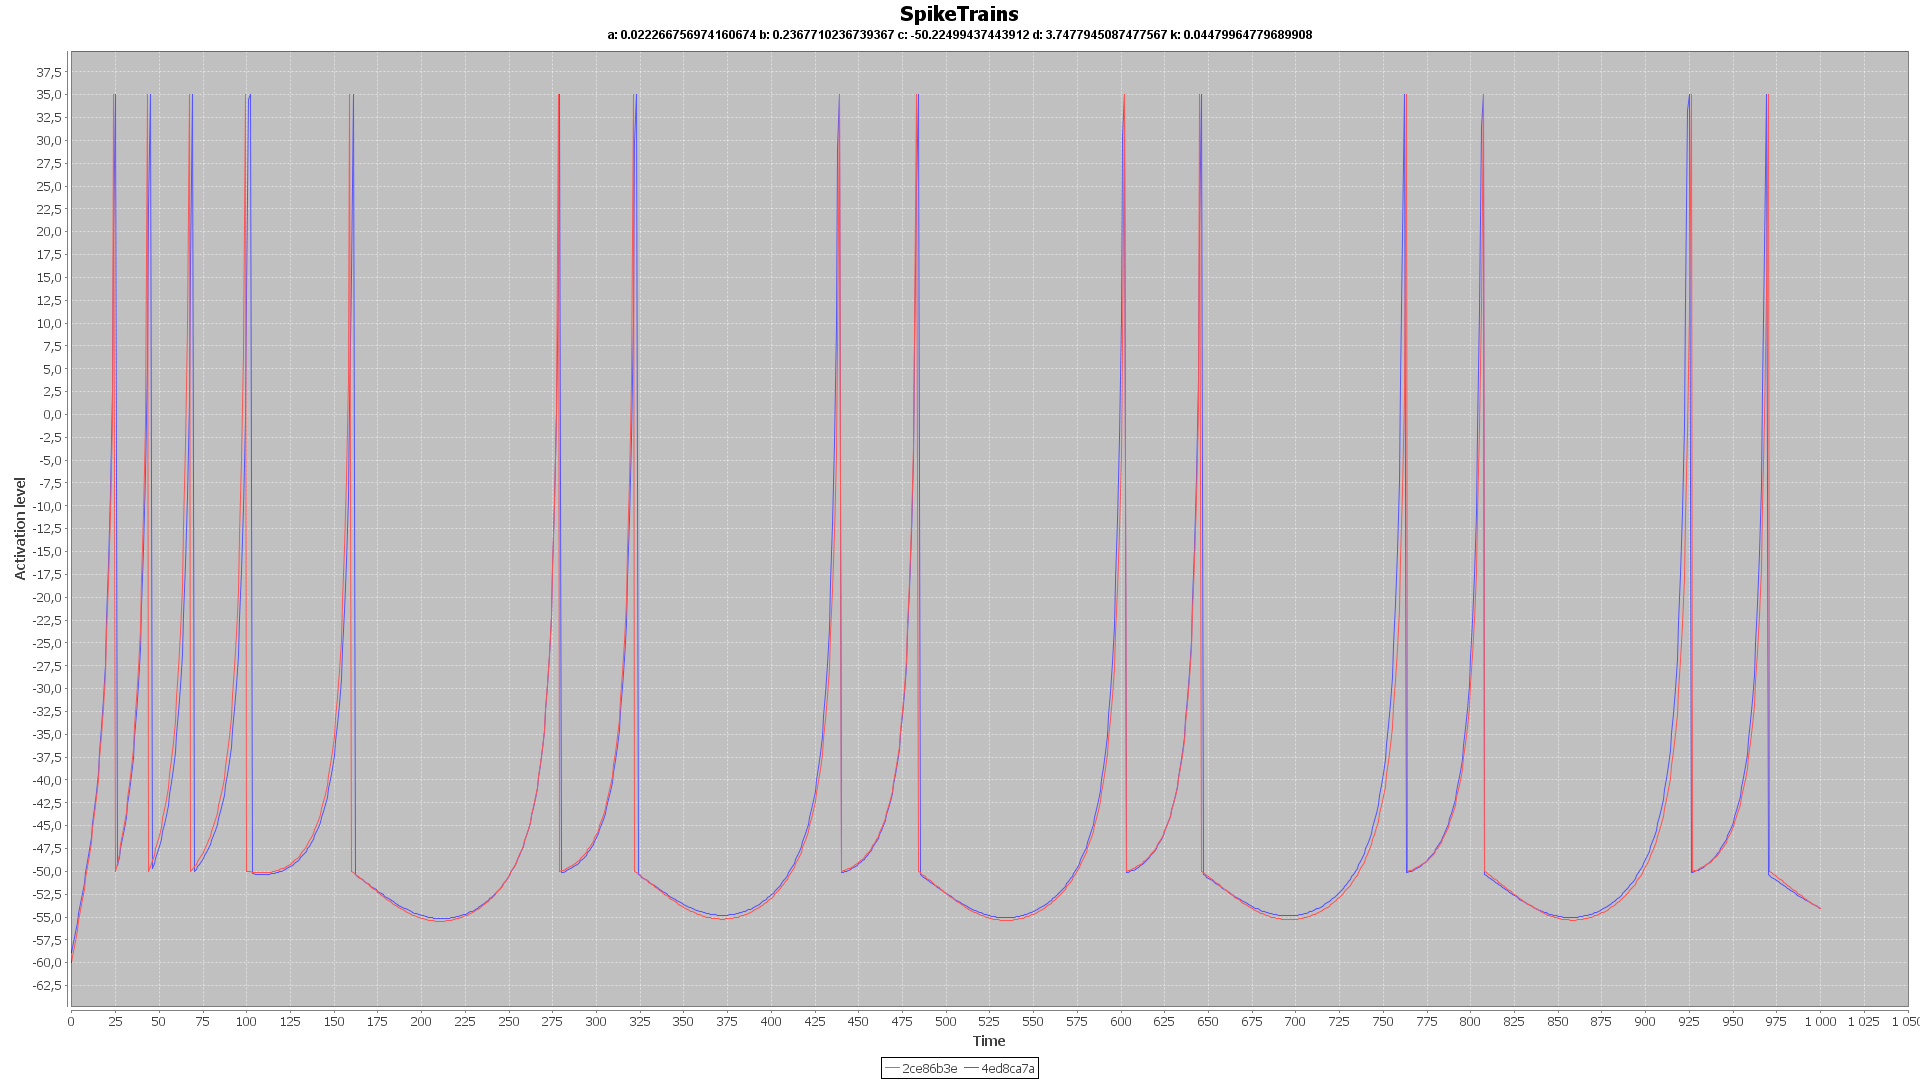
\includegraphics[width=\linewidth]{./../images/izzy2/wave/plot.png}

						\label{fig:sub6a}
					\end{subfigure}%
					\begin{subfigure}{.5\textwidth}
						\centering
						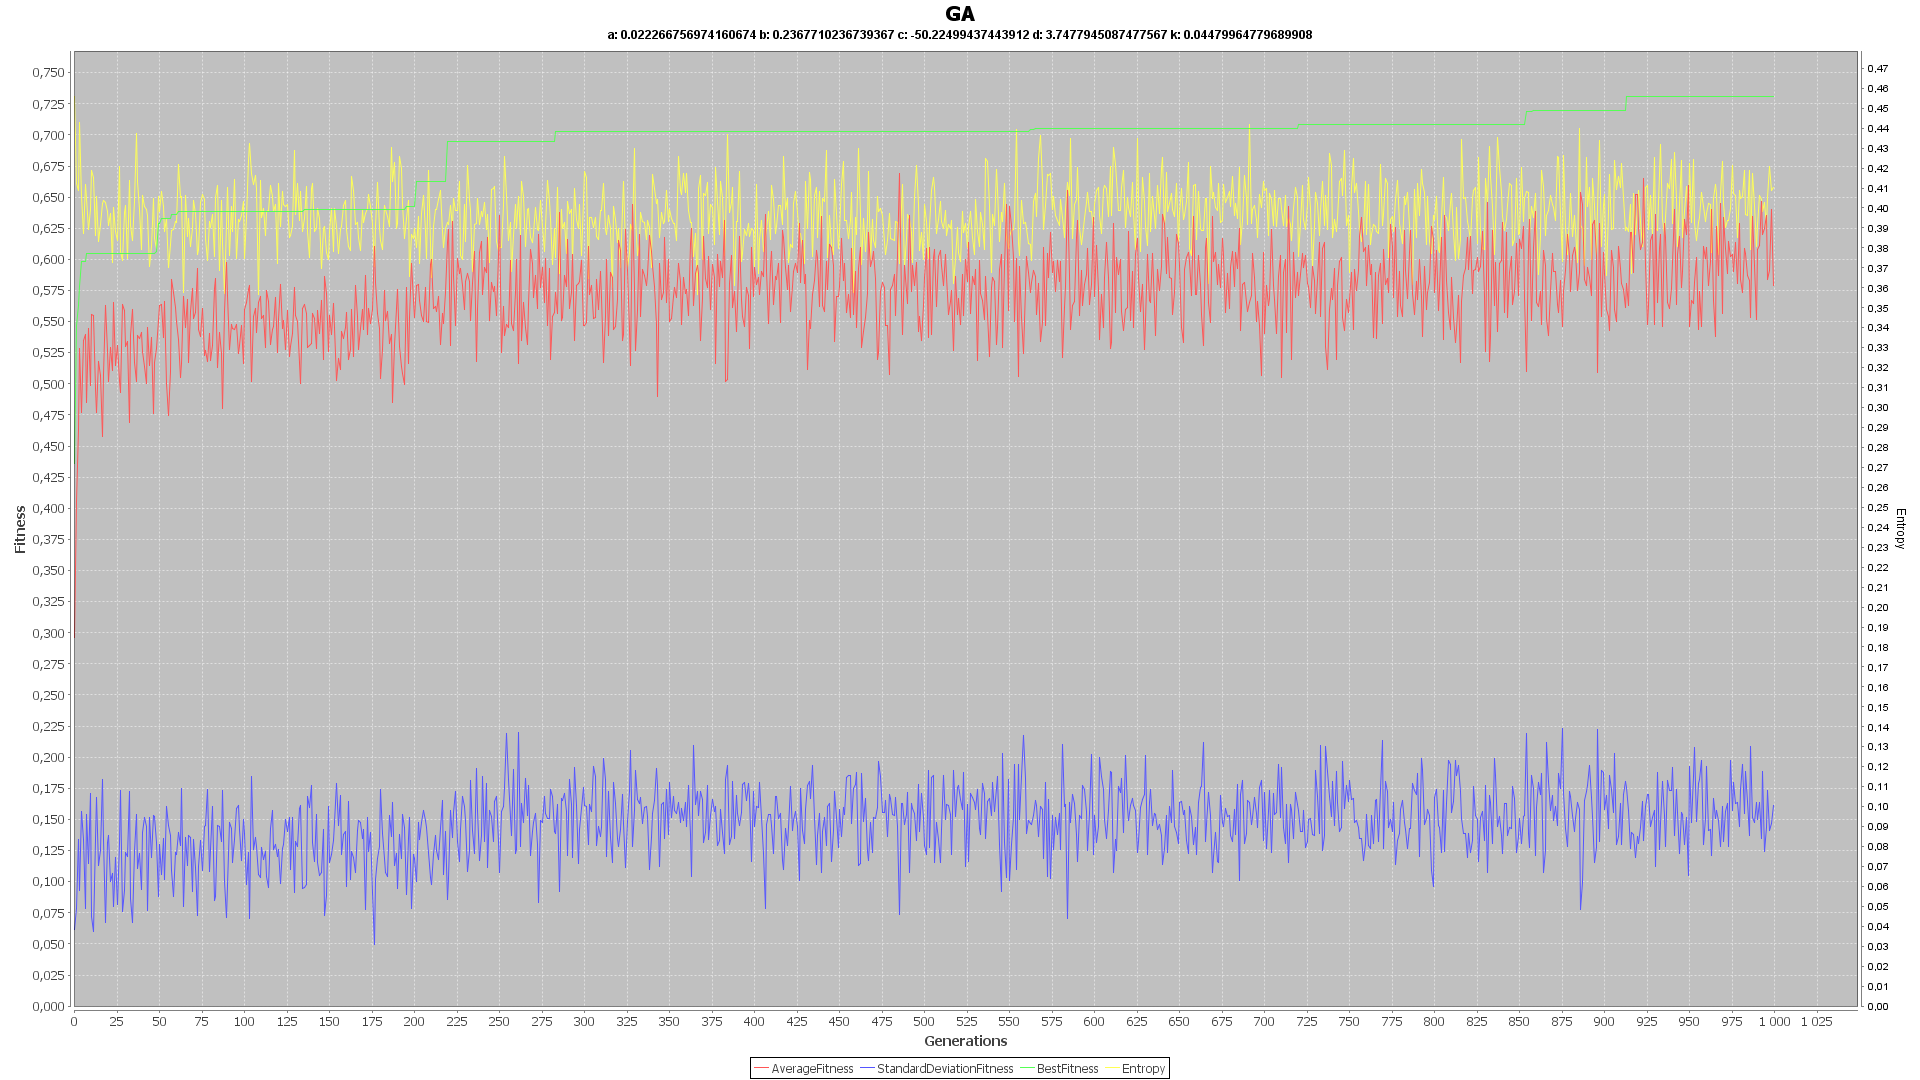
\includegraphics[width=\linewidth]{./../images/izzy2/wave/prog.png}
						
						\label{fig:sub6b}
					\end{subfigure}
					
					\label{fig:plot6}
			\end{figure}
		\subsubsection{Parameters}
			\begin{table}[H]
				\begin{tabular}{lll}
					SDM & Best Fitness & Parameter\\\hline\hline
					SpikeTime & $0.9444$ & $[a,b,c,d,k]= [0.0211,0.2756, -49.91, 3.967, 0.0450]$\\
					SpikeInterval & $0.8888$ & $[a,b,c,d,k]= [0.0261,0.1685, -49.89, 3.9535, 0.0451]$\\
					Waveform & $0.7306$ & $[a,b,c,d,k]= [0.0223,0.2368, -50.22, 3.748, 0.0448]$\\
				\end{tabular}
				\caption{The best found solutions for izzy 2 given the SDM}
			\end{table}
		
	\subsection{Izzy 3}
		\subsubsection{Spike time distance metric}
			\begin{figure}[H]
				\centering
					\begin{subfigure}{.5\textwidth}
						\centering
						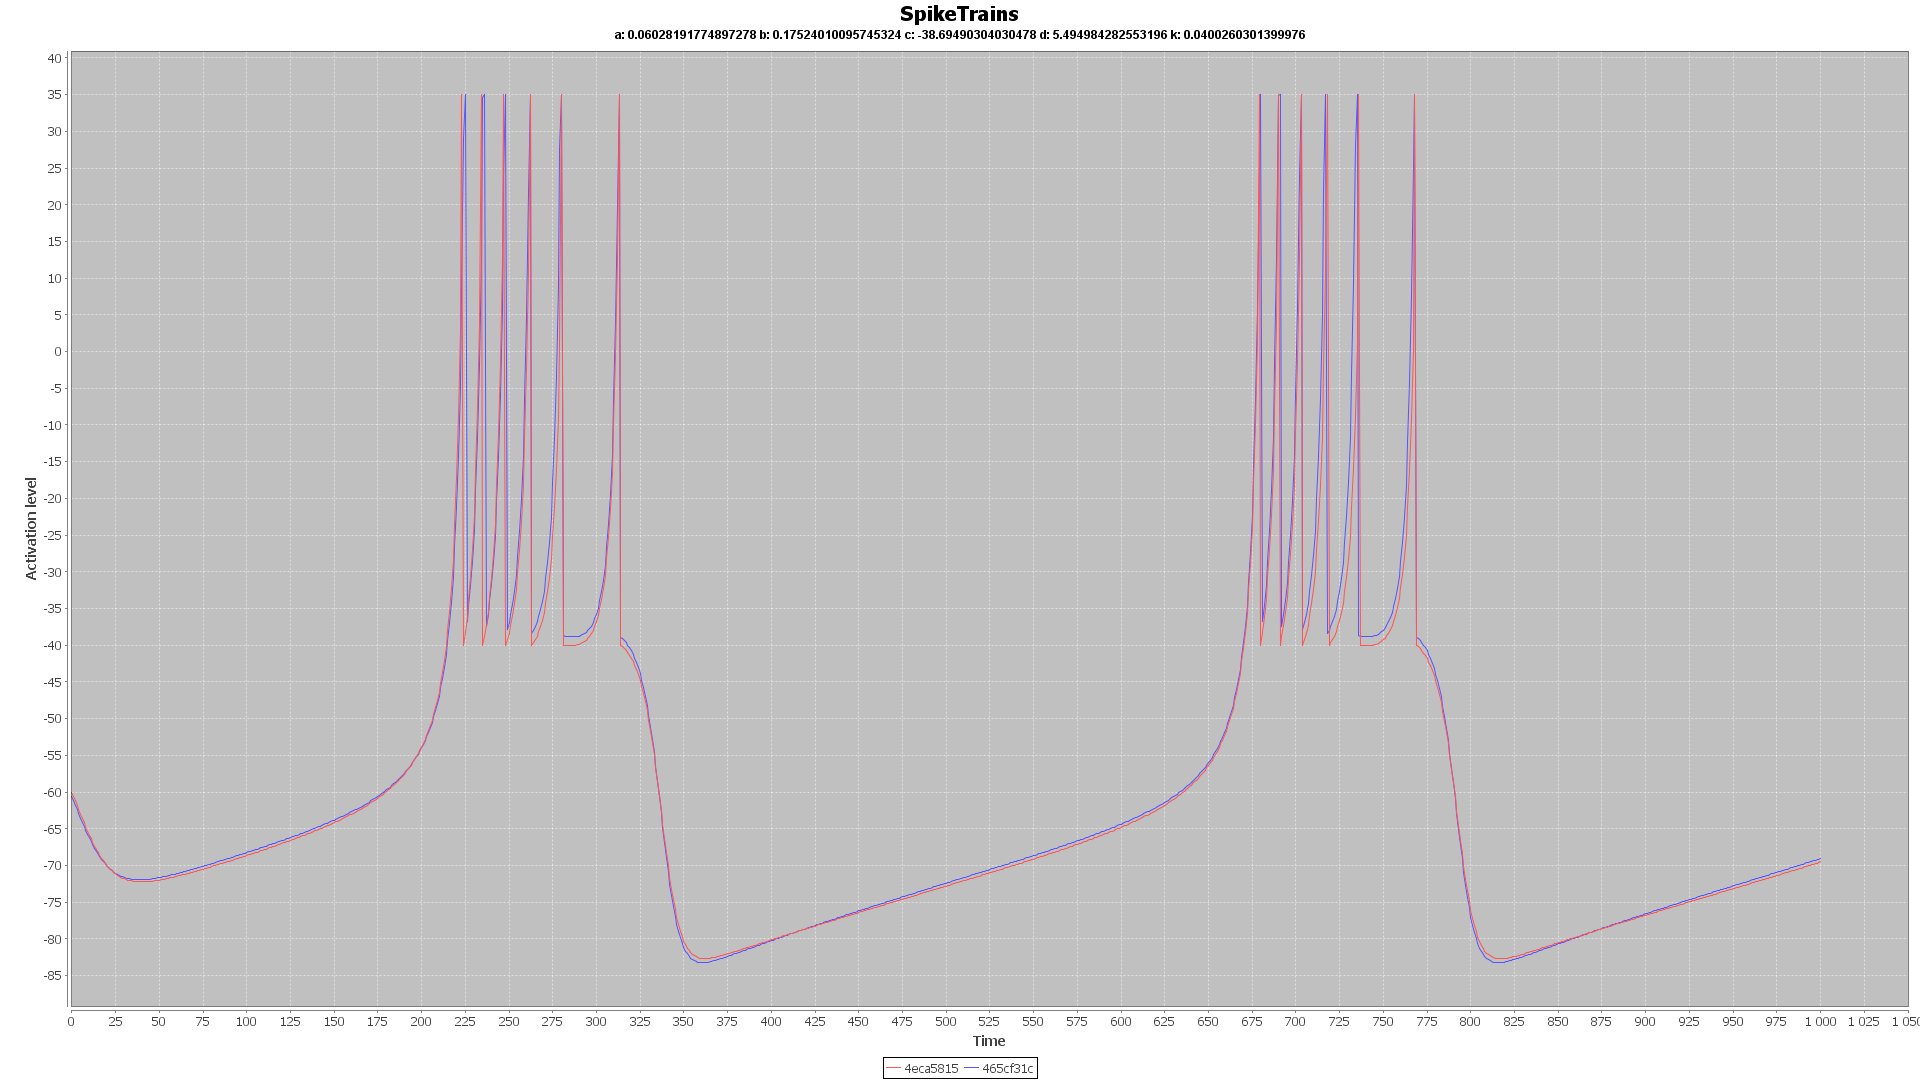
\includegraphics[width=\linewidth]{./../images/izzy3/time/plot.png}
						
						\label{fig:sub7a}
					\end{subfigure}%
					\begin{subfigure}{.5\textwidth}
						\centering
						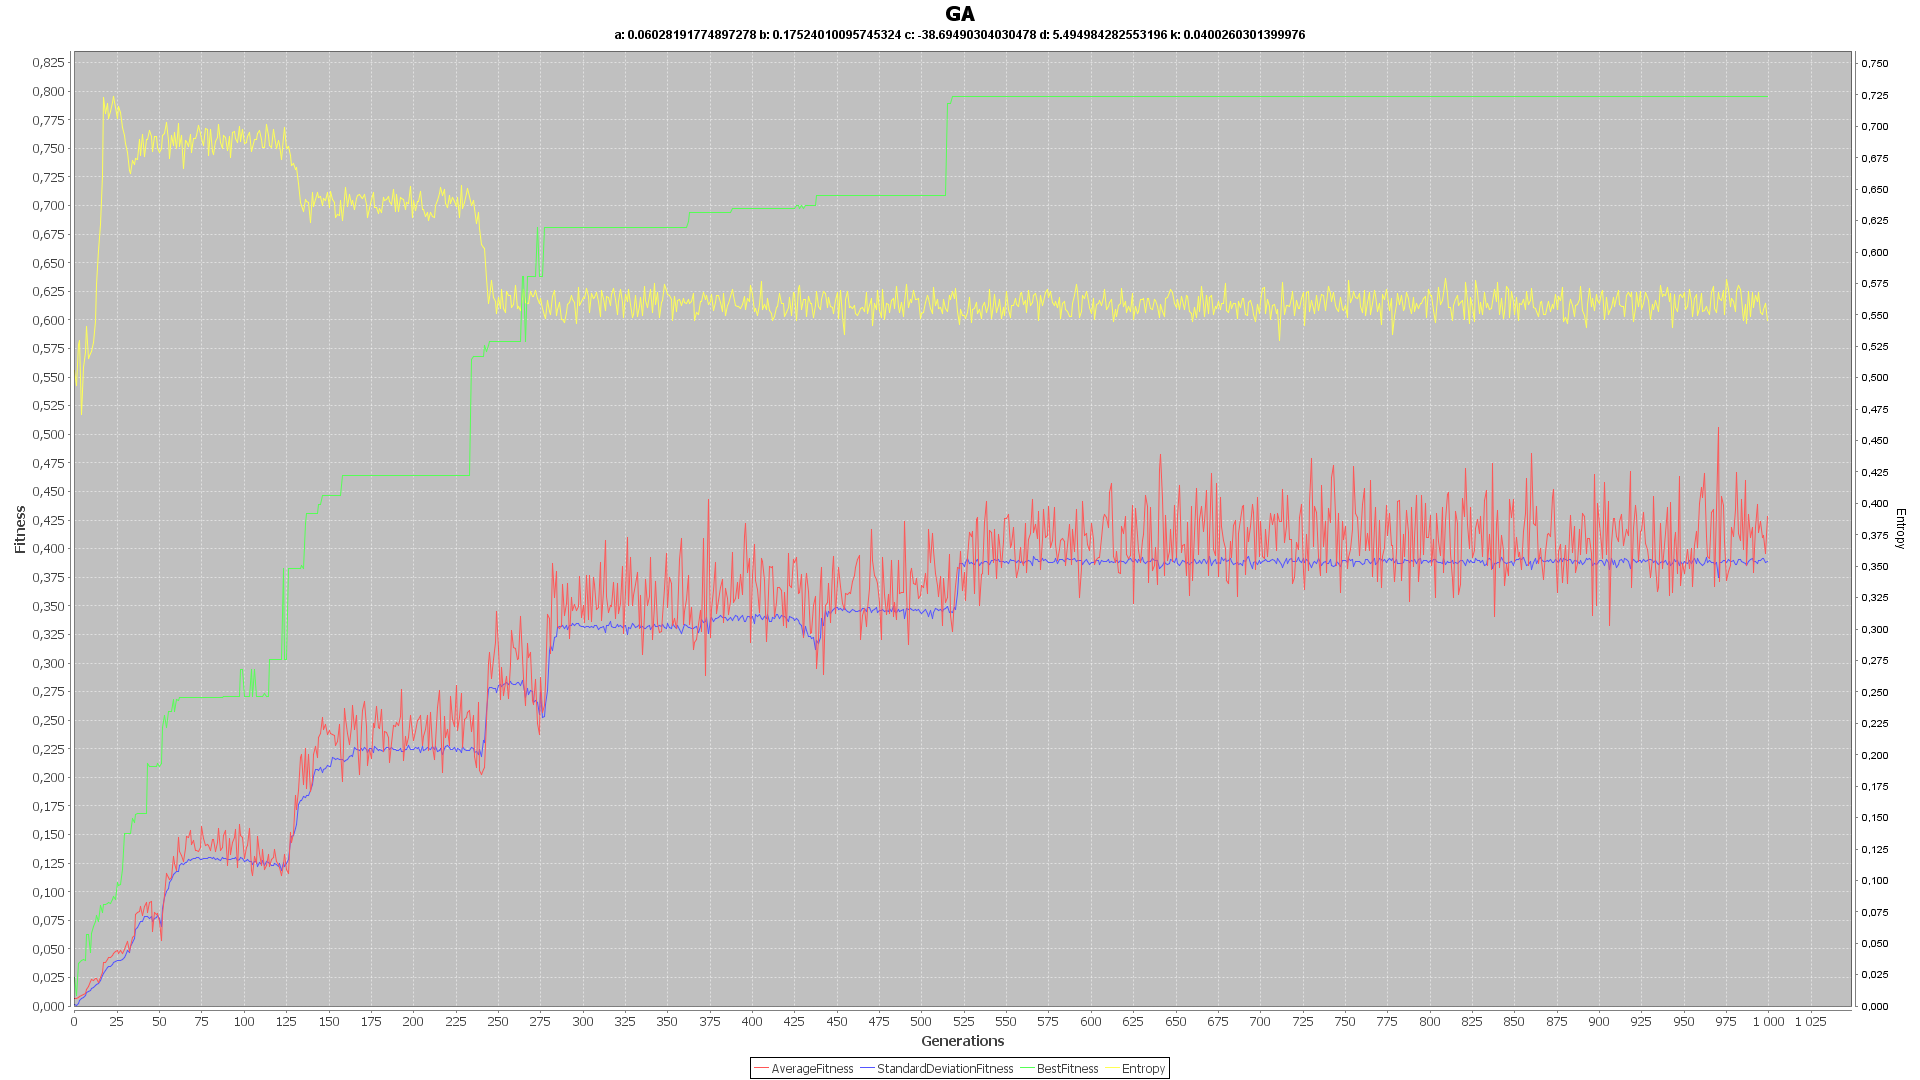
\includegraphics[width=\linewidth]{./../images/izzy3/time/prog.png}
						
						\label{fig:sub7b}
					\end{subfigure}
					
					\label{fig:plot7}
			\end{figure}
			
		\subsubsection{Spike interval distance metric}
			\begin{figure}[H]
				\centering
					\begin{subfigure}{.5\textwidth}
						\centering
						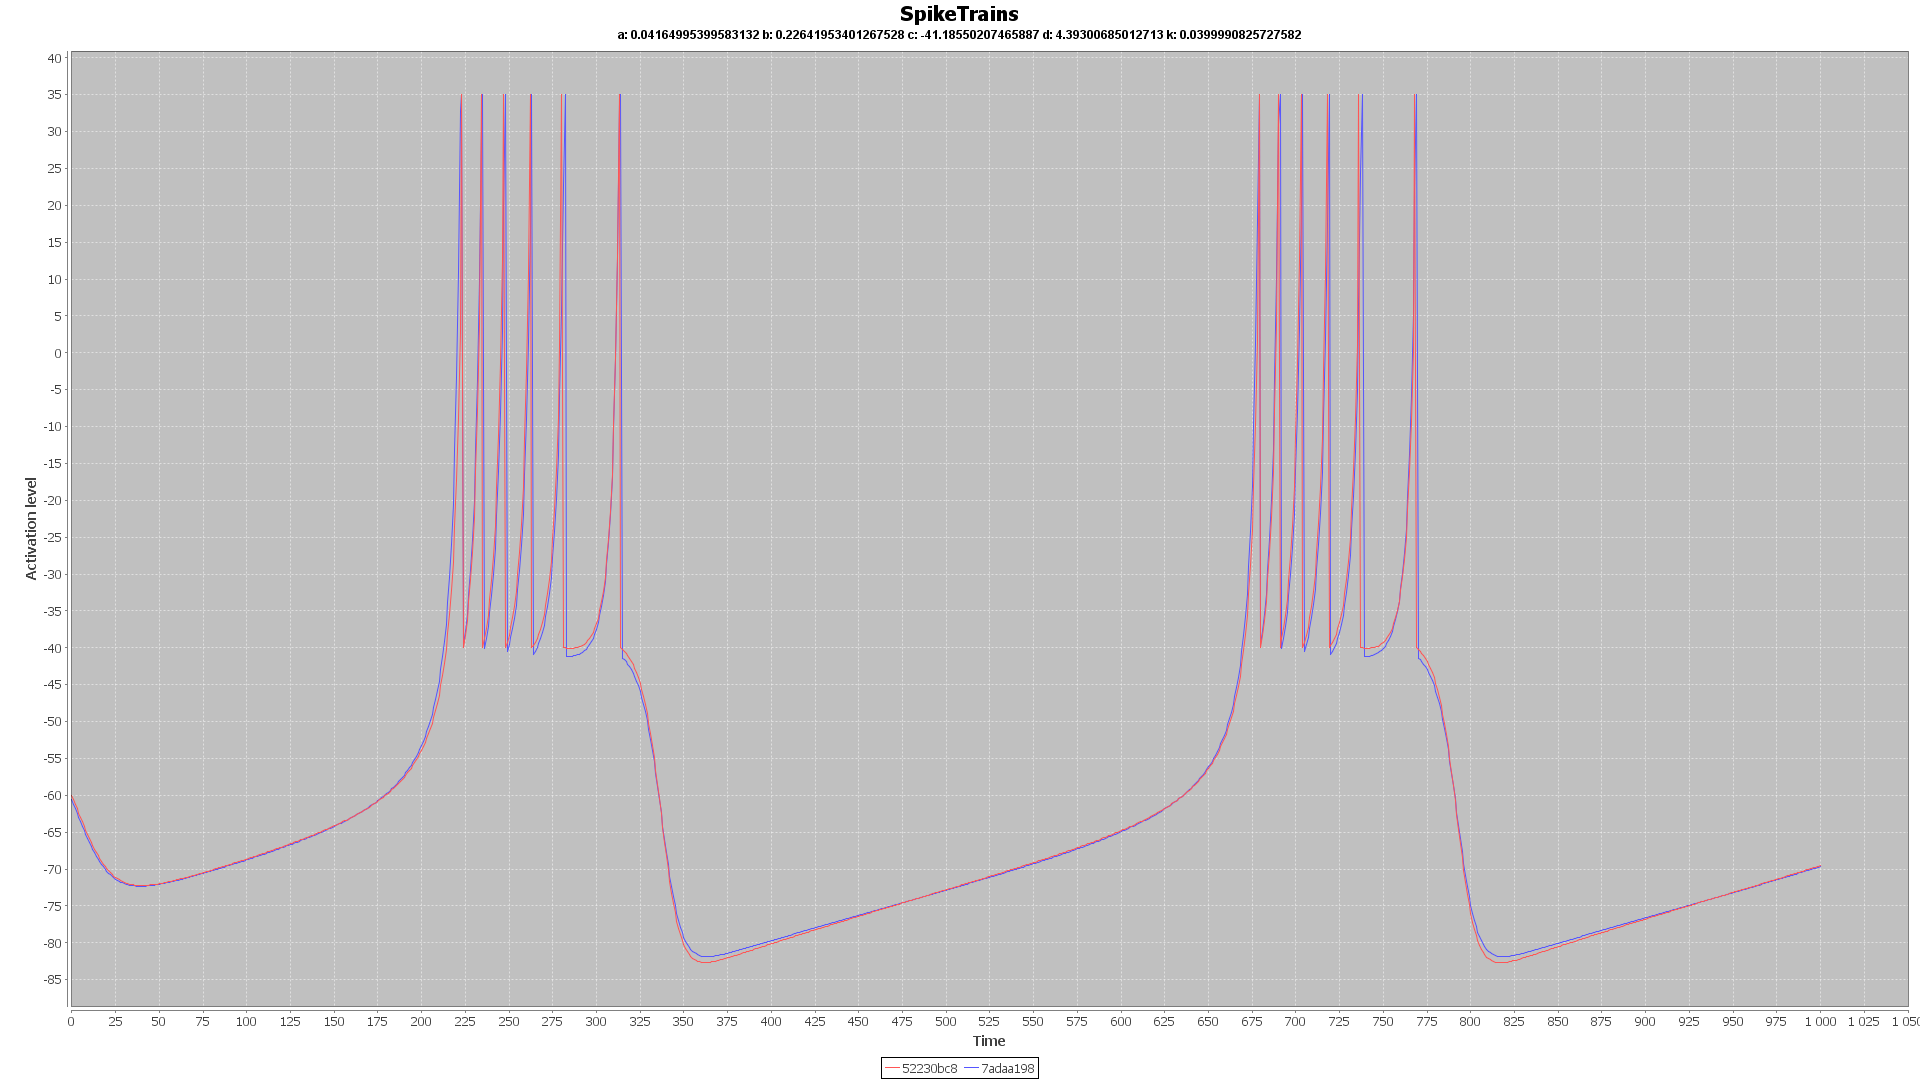
\includegraphics[width=\linewidth]{./../images/izzy3/interval/plot.png}
						
						\label{fig:sub8a}
					\end{subfigure}%
					\begin{subfigure}{.5\textwidth}
						\centering
						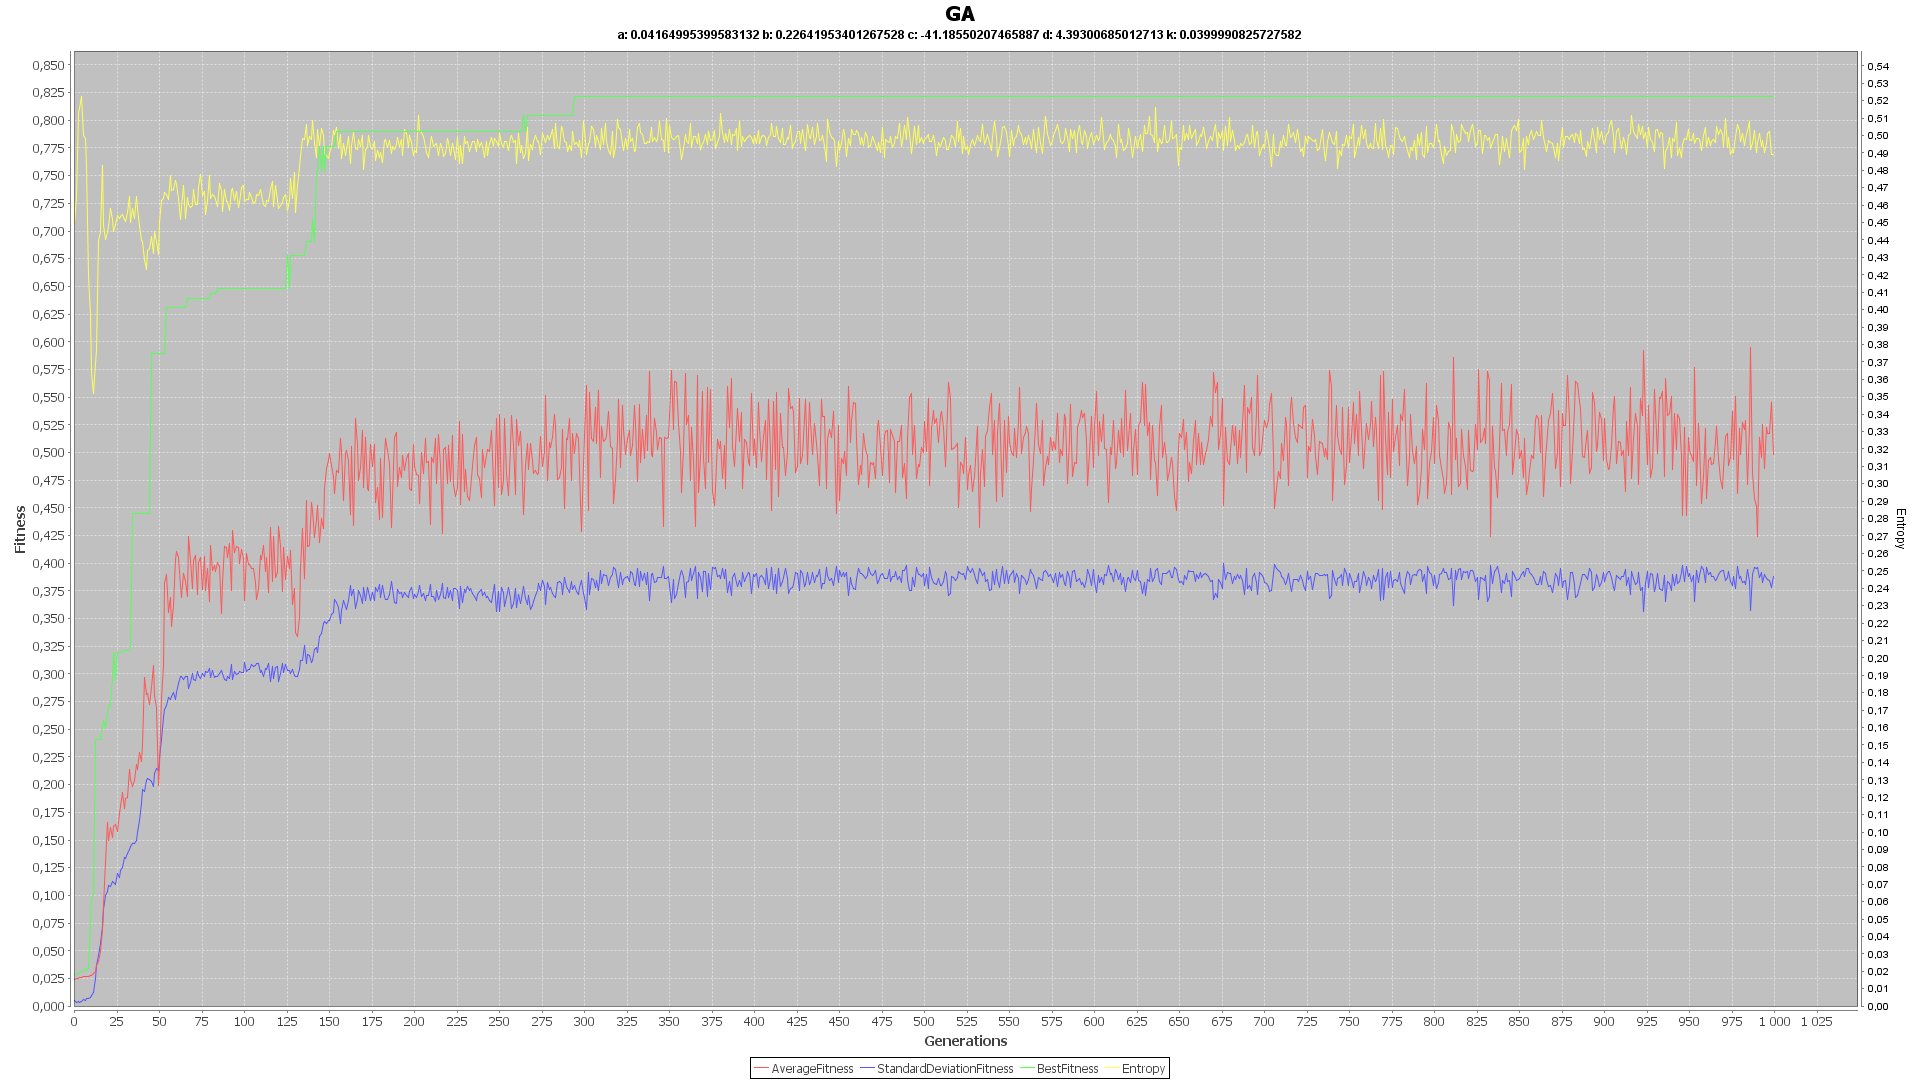
\includegraphics[width=\linewidth]{./../images/izzy3/interval/prog.png}
						
						\label{fig:sub8b}
					\end{subfigure}
					
					\label{fig:test}
			\end{figure}
			
		\subsubsection{Waveform distance metric}
			\begin{figure}[H]
				\centering
					\begin{subfigure}{.5\textwidth}
						\centering
						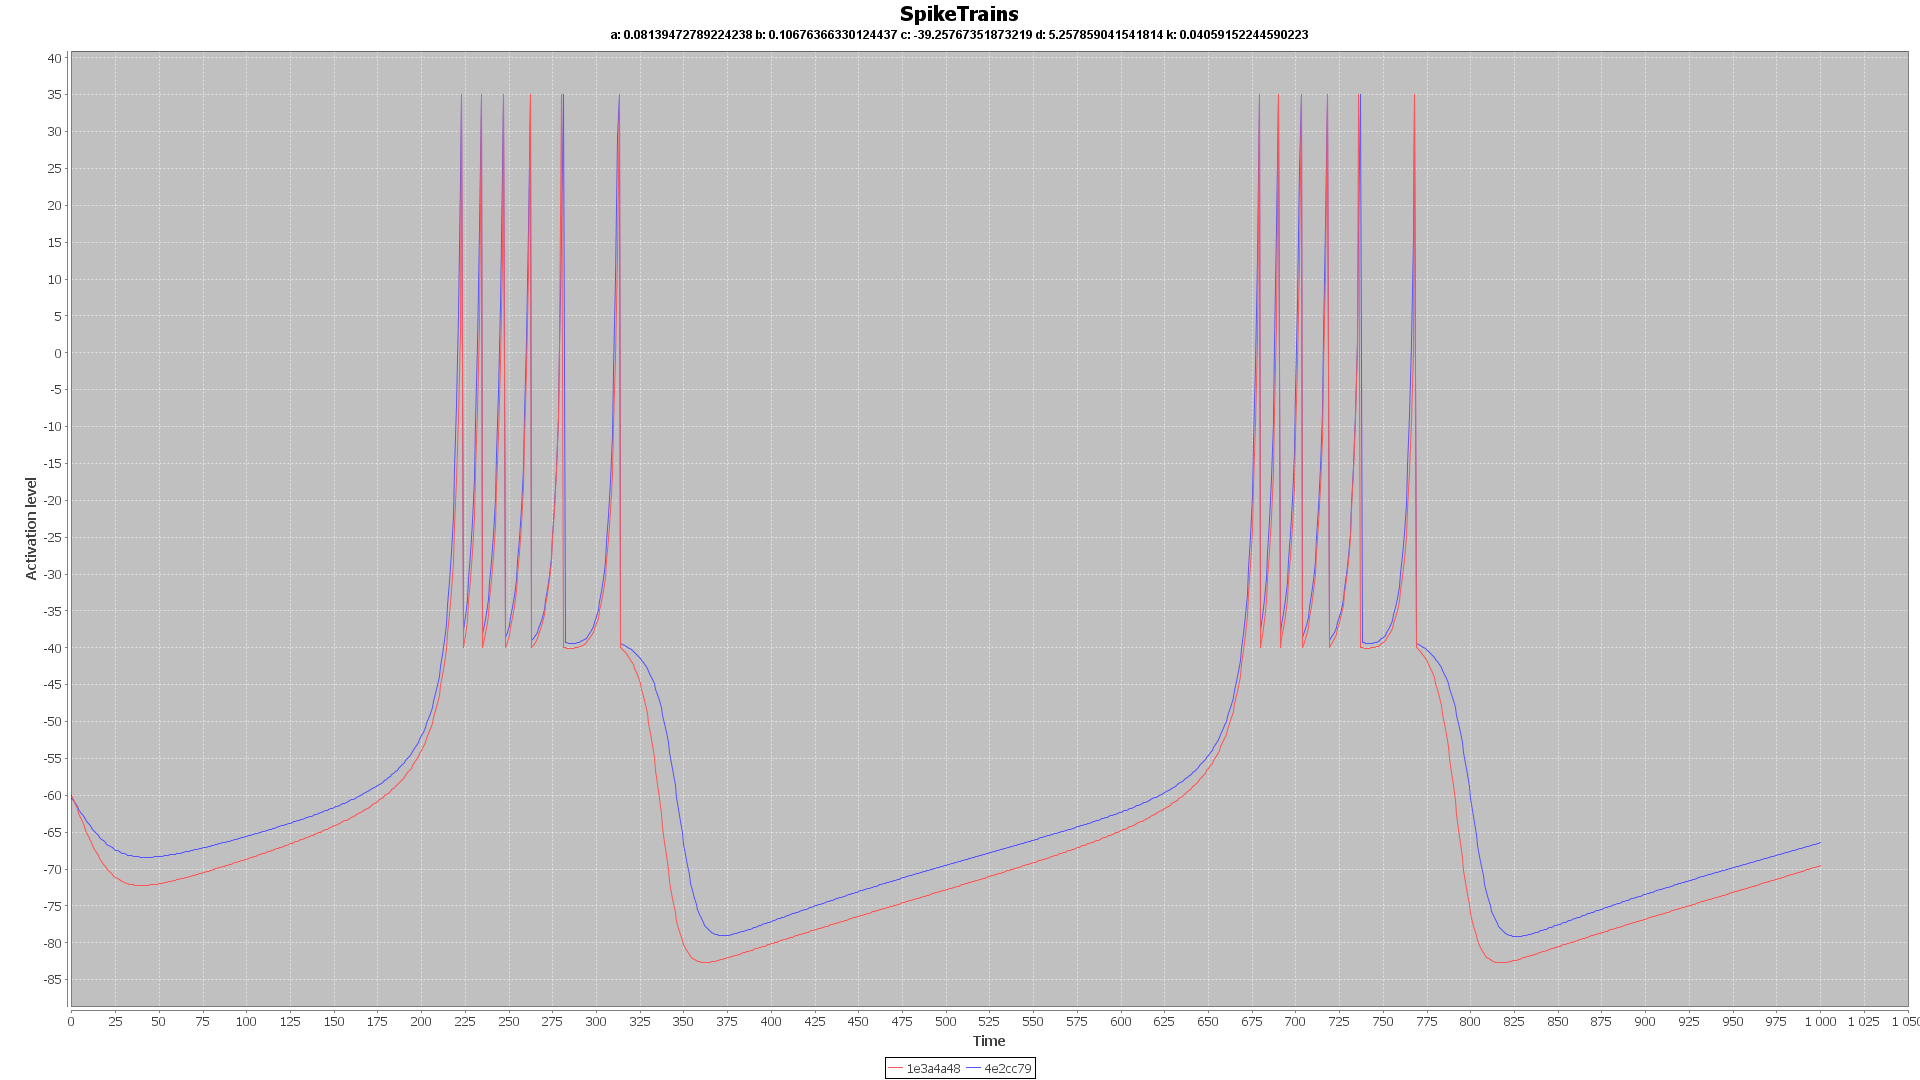
\includegraphics[width=\linewidth]{./../images/izzy3/wave/plot.png}

						\label{fig:sub9a}
					\end{subfigure}%
					\begin{subfigure}{.5\textwidth}
						\centering
						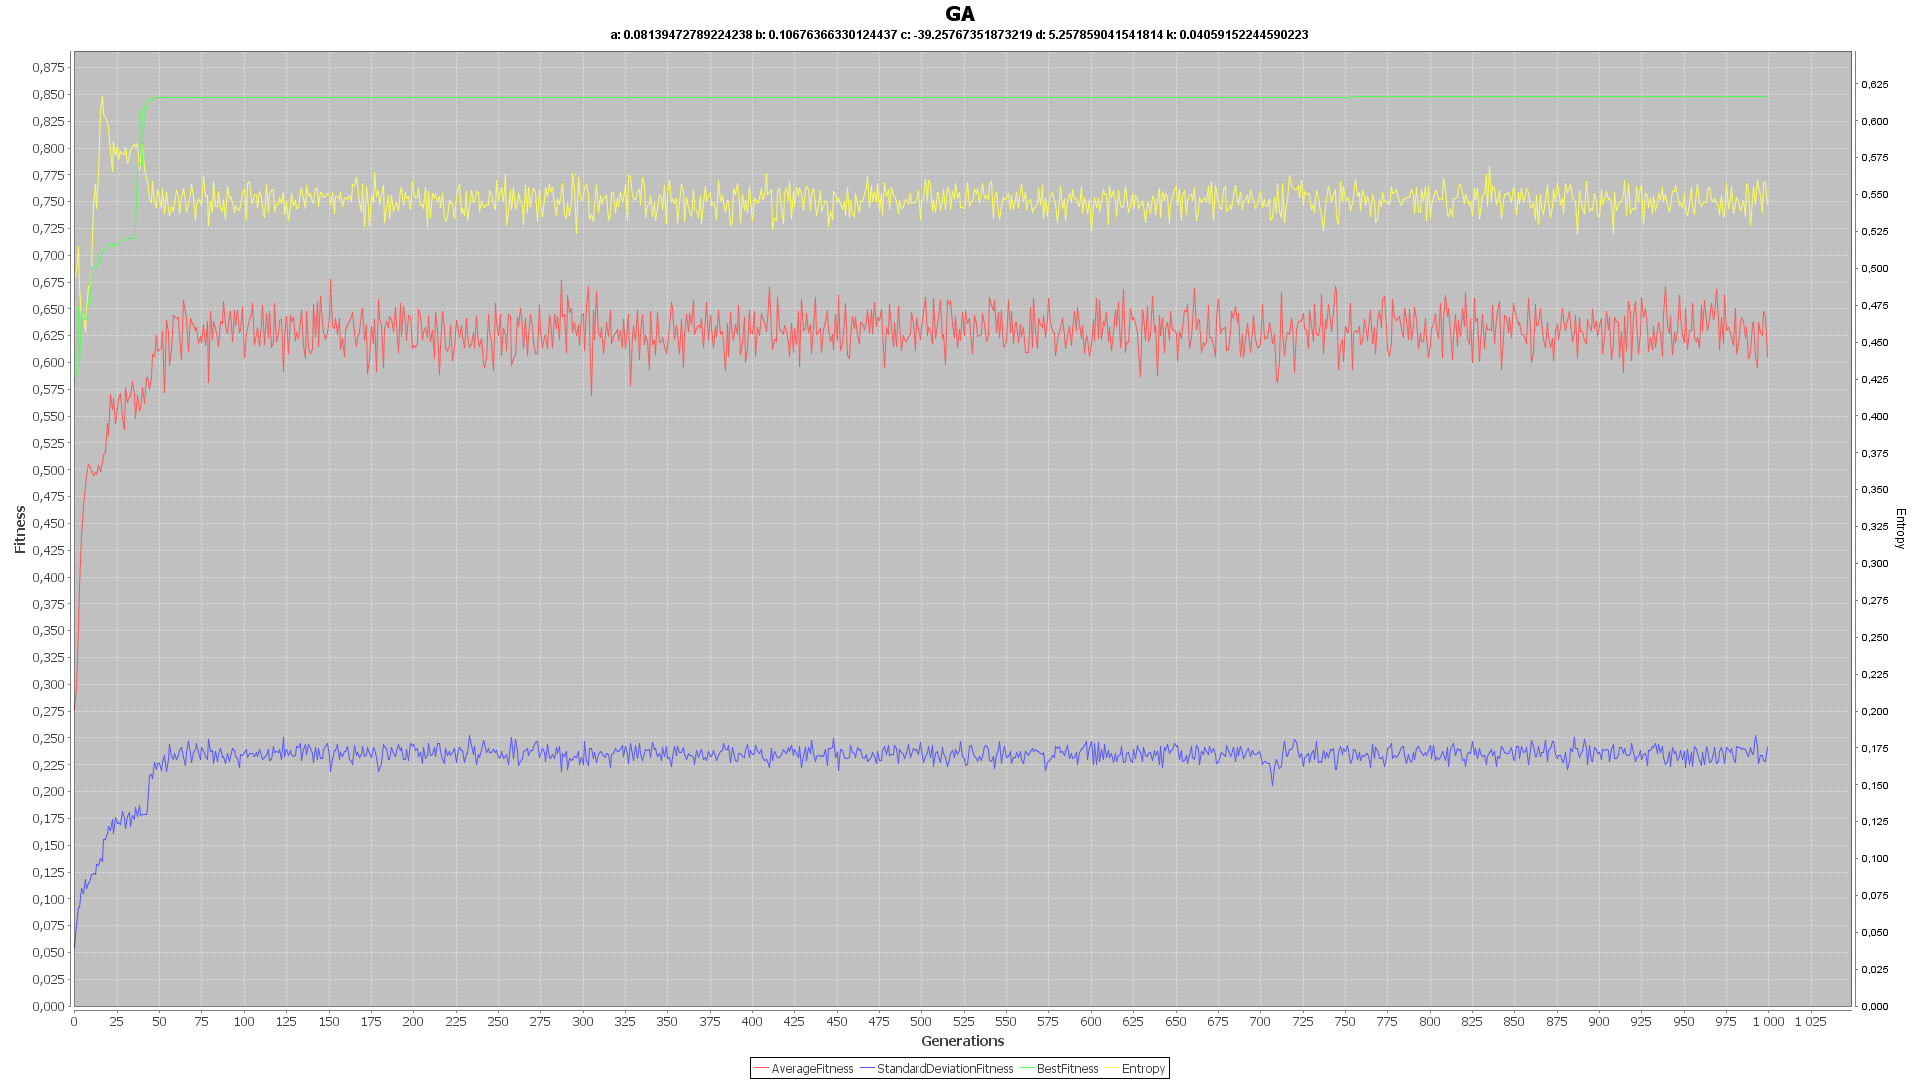
\includegraphics[width=\linewidth]{./../images/izzy3/wave/prog.png}
						
						\label{fig:sub9b}
					\end{subfigure}
					
					\label{fig:plot9}
			\end{figure}
		\subsubsection{Parameters}
			\begin{table}[H]
				\begin{tabular}{lll}
					SDM & Best Fitness & Parameter\\\hline\hline
					SpikeTime & $0.7952$ & $[a,b,c,d,k]= [0.0603,0.1752, -38.69, 5.4949, 0.0400]$\\
					SpikeInterval & $0.8213$ & $[a,b,c,d,k]= [0.0416,0.2264, -41.19, 4.3930, 0.0399]$\\
					Waveform & $0.8478$ & $[a,b,c,d,k]= [0.0814,0.1068, -39.26, 5.258, 0.0406]$\\
				\end{tabular}
				\caption{The best found solutions for izzy 3 given the SDM}
			\end{table}
	\subsection{Izzy 4}
		\subsubsection{Spike time distance metric}
			\begin{figure}[H]
				\centering
					\begin{subfigure}{.5\textwidth}
						\centering
						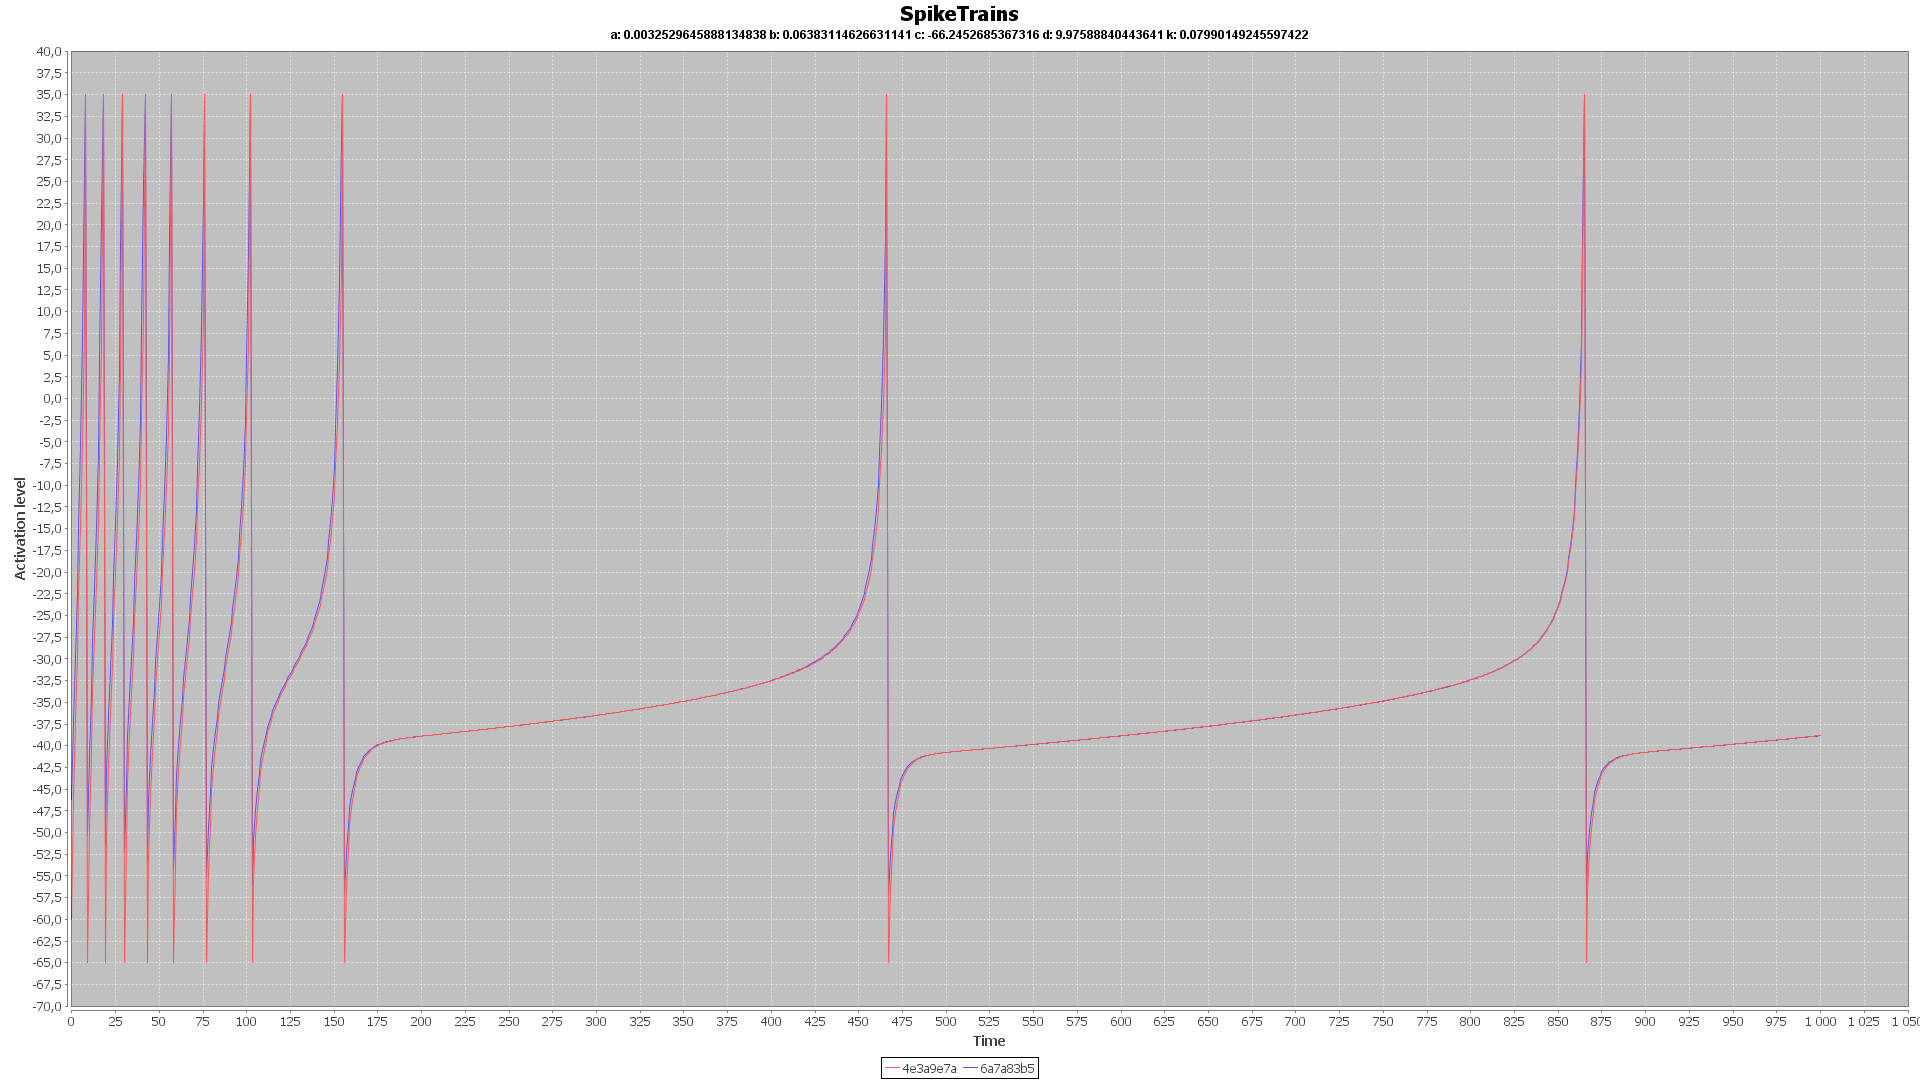
\includegraphics[width=\linewidth]{./../images/izzy4/time/plot.png}
						
						\label{fig:sub10a}
					\end{subfigure}%
					\begin{subfigure}{.5\textwidth}
						\centering
						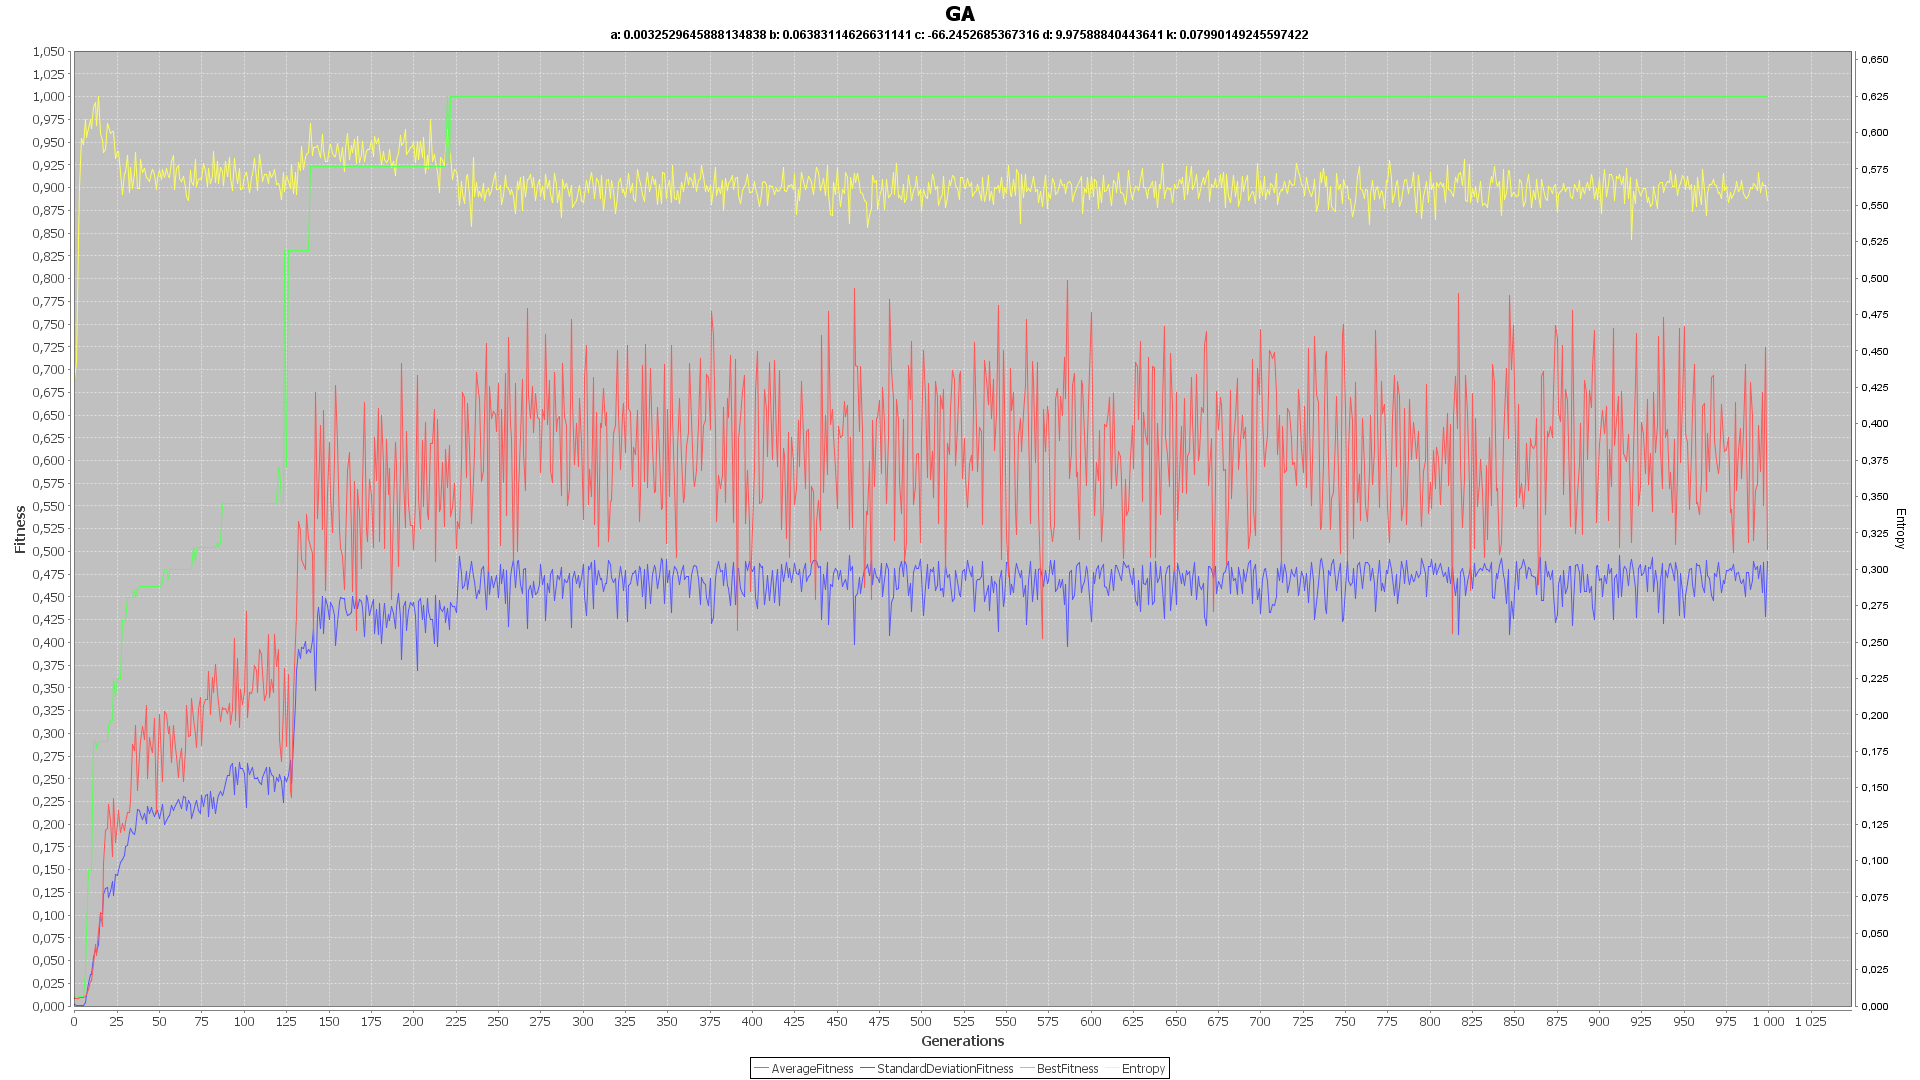
\includegraphics[width=\linewidth]{./../images/izzy4/time/prog.png}
						
						\label{fig:sub10b}
					\end{subfigure}
					
					\label{fig:plot10}
			\end{figure}
			
		\subsubsection{Spike interval distance metric}
			\begin{figure}[H]
				\centering
					\begin{subfigure}{.5\textwidth}
						\centering
						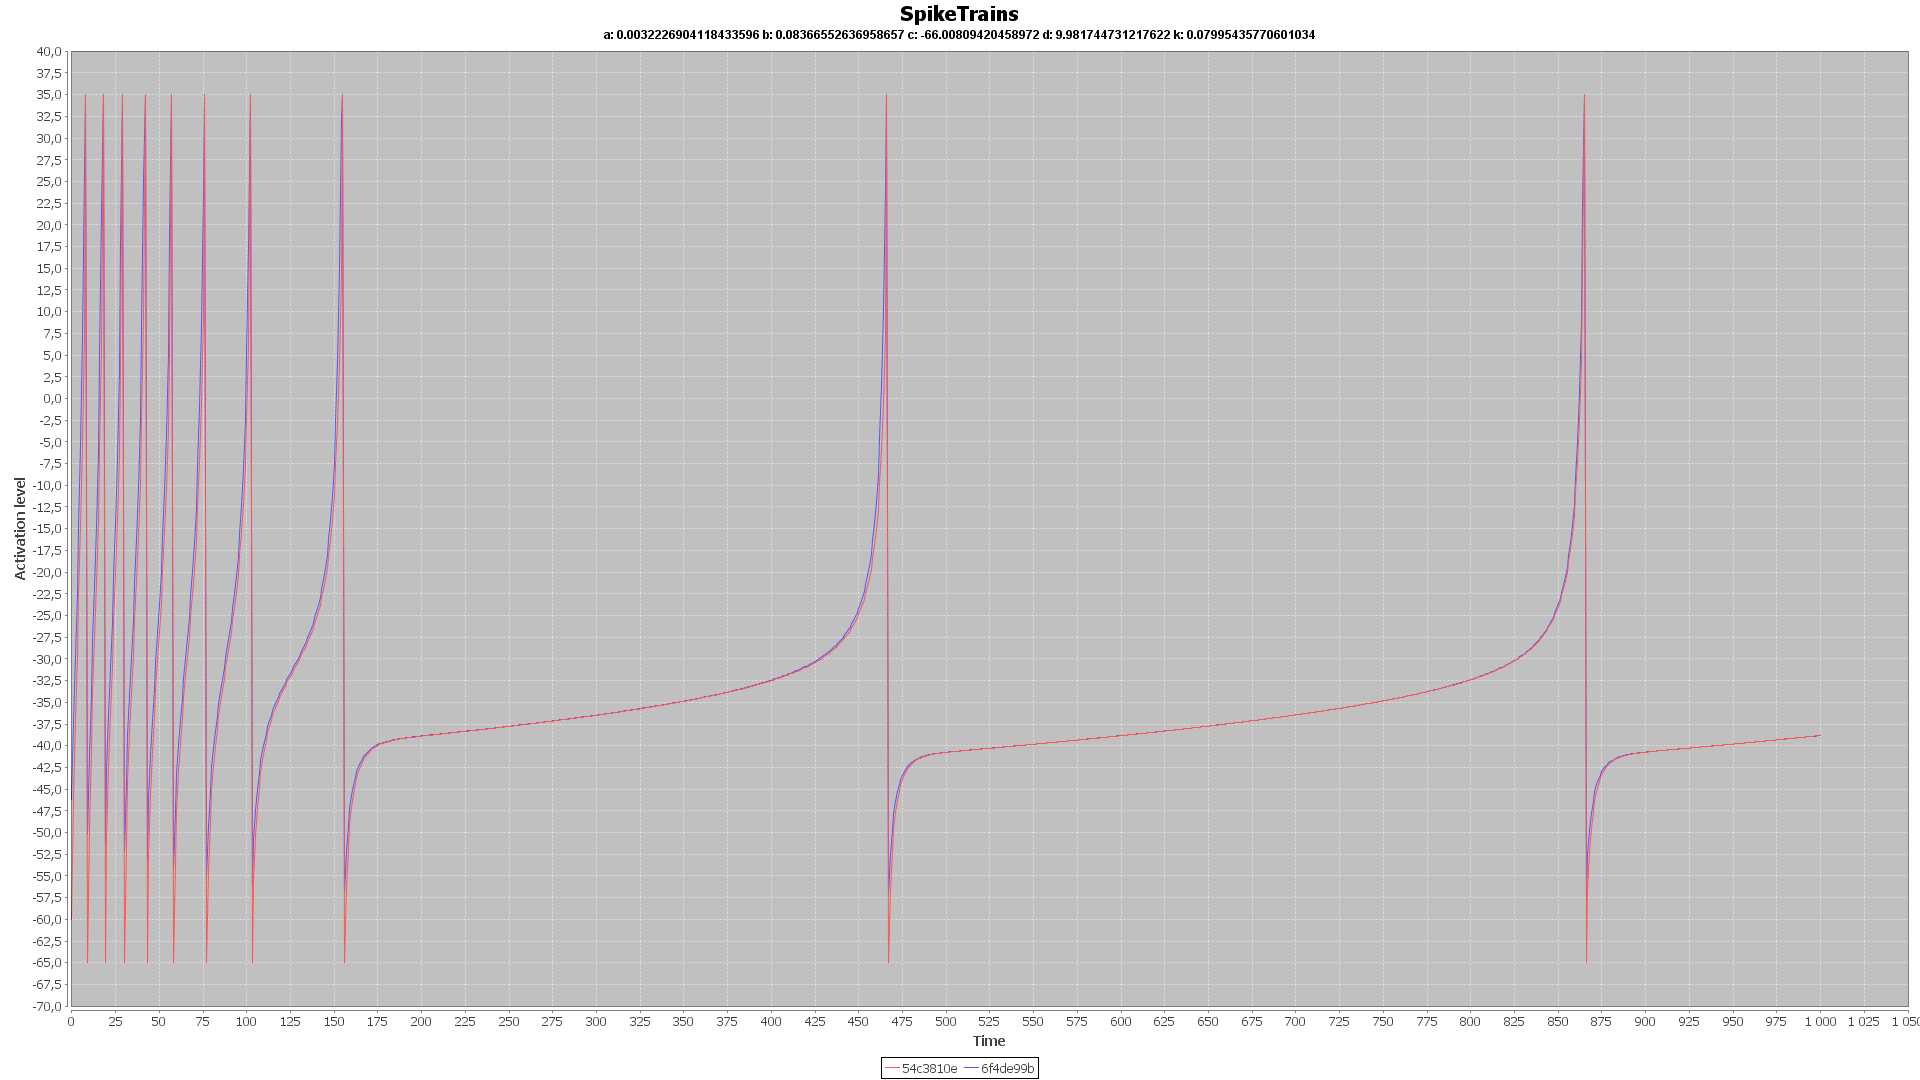
\includegraphics[width=\linewidth]{./../images/izzy4/interval/plot.png}
						
						\label{fig:sub11a}
					\end{subfigure}%
					\begin{subfigure}{.5\textwidth}
						\centering
						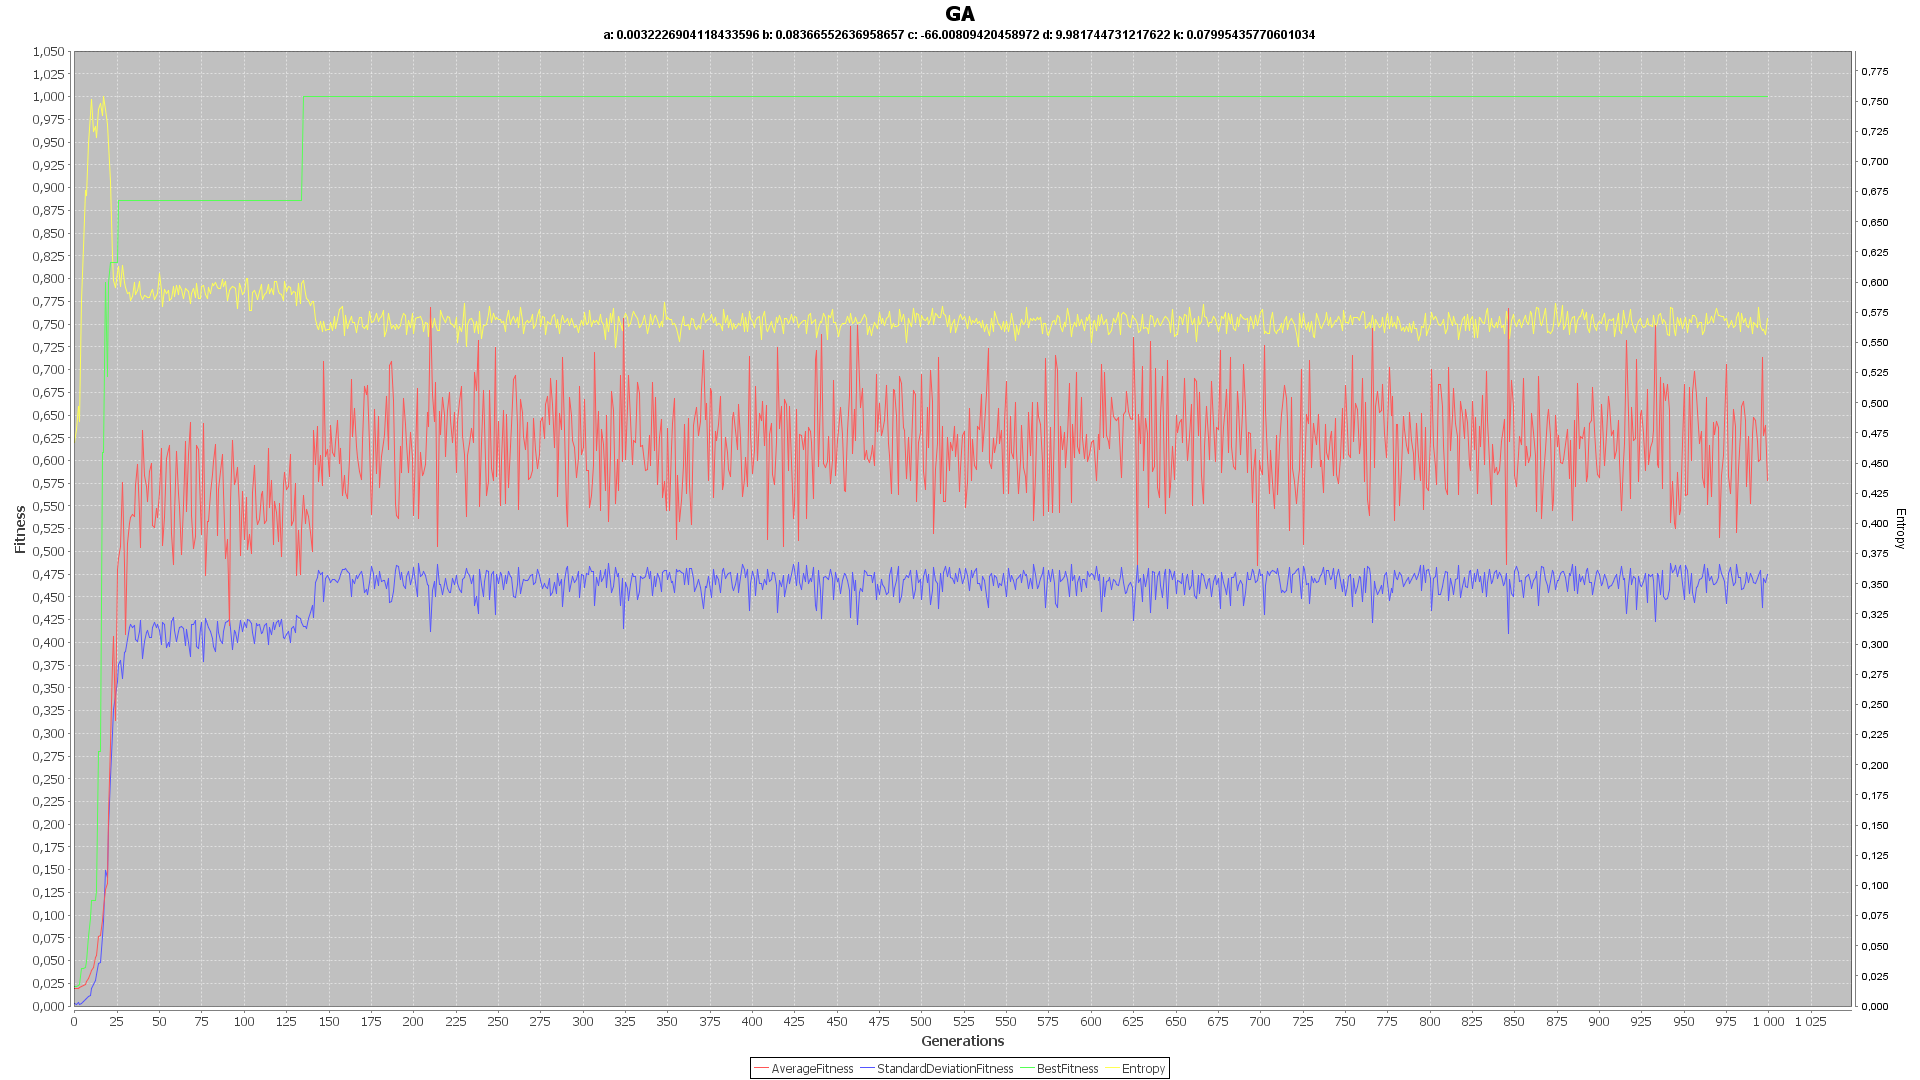
\includegraphics[width=\linewidth]{./../images/izzy4/interval/prog.png}
						
						\label{fig:sub11b}
					\end{subfigure}
					
					\label{fig:plot11}
			\end{figure}
		\subsubsection{Waveform distance metric}
			\begin{figure}[H]
				\centering
					\begin{subfigure}{.5\textwidth}
						\centering
						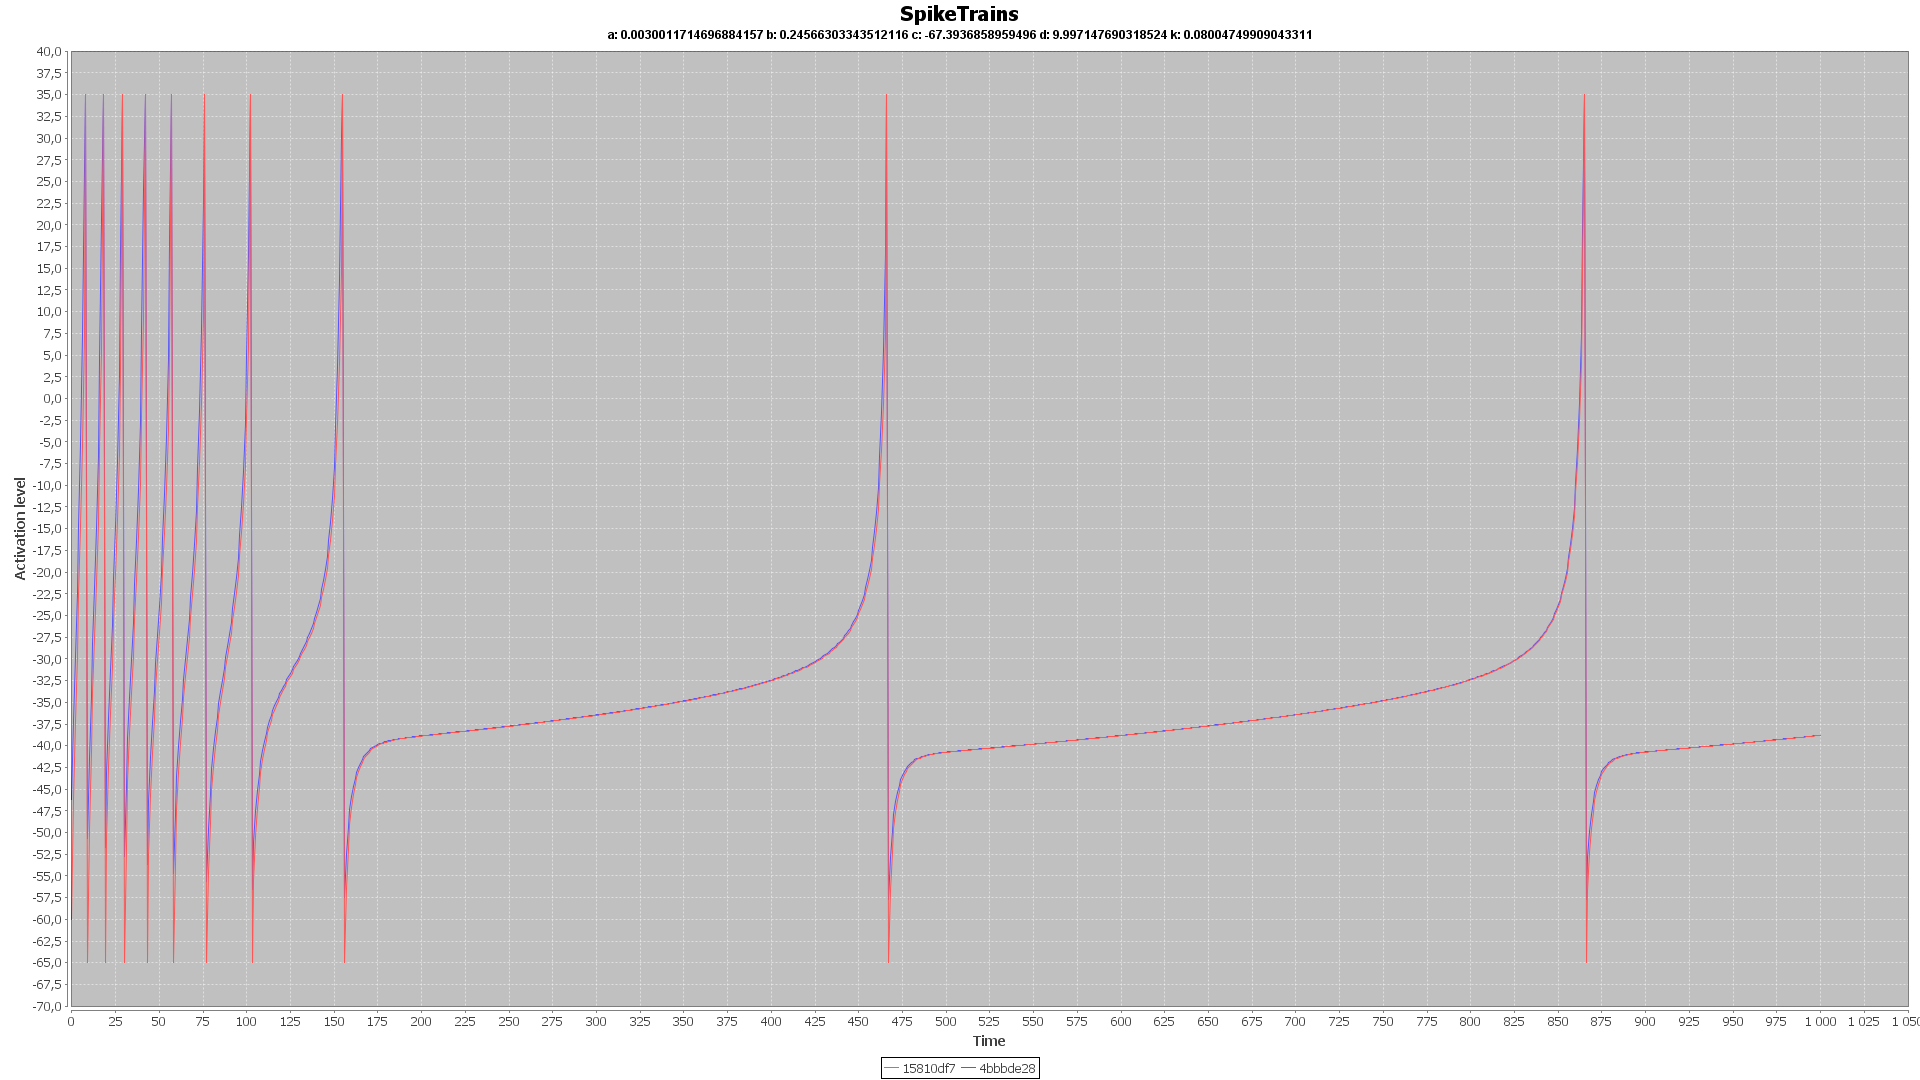
\includegraphics[width=\linewidth]{./../images/izzy4/wave/plot.png}

						\label{fig:sub12a}
					\end{subfigure}%
					\begin{subfigure}{.5\textwidth}
						\centering
						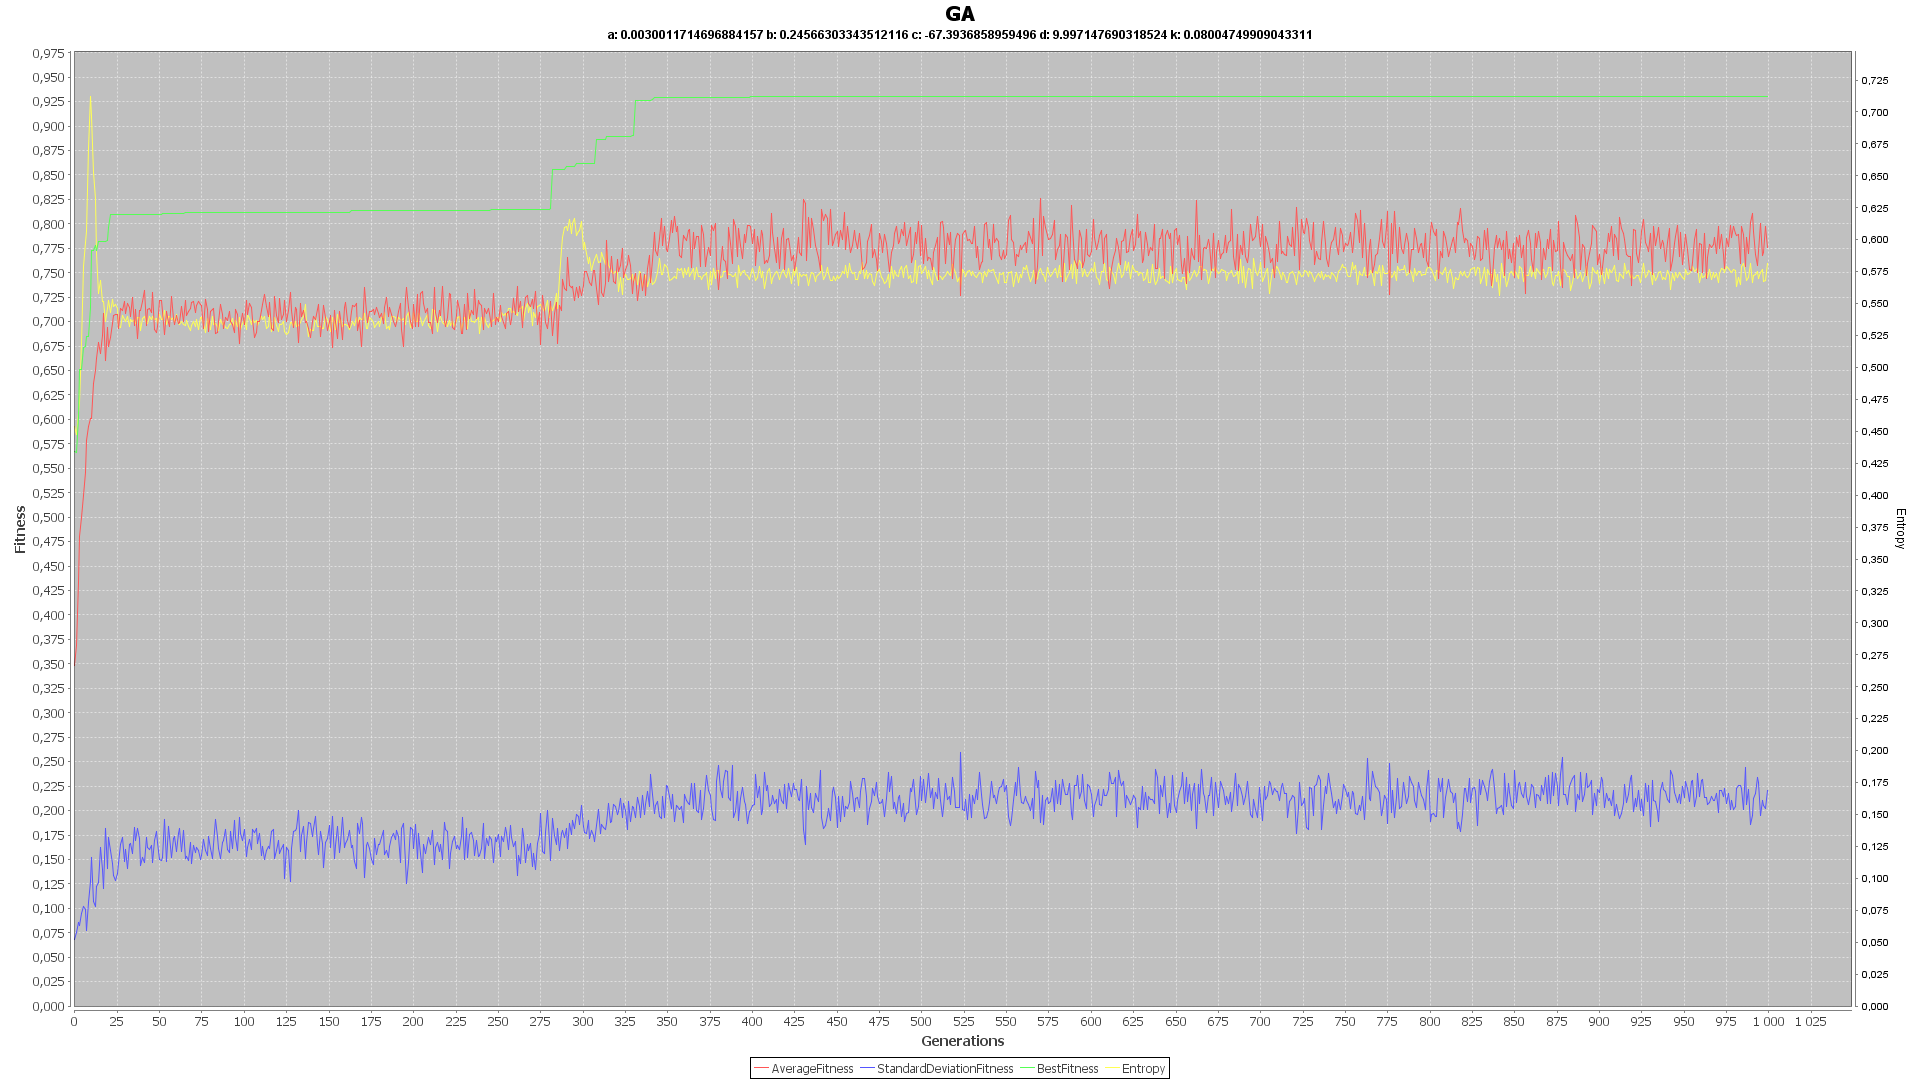
\includegraphics[width=\linewidth]{./../images/izzy4/wave/prog.png}
						
						\label{fig:sub12b}
					\end{subfigure}
					
					\label{fig:plot12}
			\end{figure}
		\subsubsection{Parameters}
			\begin{table}[H]
				\begin{tabular}{lll}
					SDM & Best Fitness & Parameter\\\hline\hline
					SpikeTime & $1.0$ & $[a,b,c,d,k]= [0.0033,0.0638, -66.25, 9.9759, 0.0799]$\\
					SpikeInterval & $1.0$ & $[a,b,c,d,k]= [0.0032,0.0837, -66.01, 9.9817, 0.0799]$\\
					Waveform & $0.93$ & $[a,b,c,d,k]= [0.0030,0.2457, -67.39, 9.997, 0.0800]$\\
				\end{tabular}
				\caption{The best found solutions for izzy 4 given the SDM}
			\end{table}
	
\section{Genotype-Phenotype mapping}\label{sec:mapping}
\section{Practical implications}\label{sec:implications}
\section{Application in other problem domains}\label{sec:applications}
\end{document}